\documentclass[a4paper]{article}

\def\npart {III}
\def\nterm {Lent}
\def\nyear {2017}
\def\nlecturer {C. E. Thomas}
\def\ncourse {The Standard Model}
\def\nofficial {https://www.damtp.cam.ac.uk/user/cet34/teaching/SM/}
\def\nlectures {MWF.9}

% Imports
\ifx \nextra \undefined
  \usepackage[pdftex,
    hidelinks,
    pdfauthor={Dexter Chua},
    pdfsubject={Cambridge Maths Notes: Part \npart\ - \ncourse},
    pdftitle={Part \npart\ - \ncourse},
  pdfkeywords={Cambridge Mathematics Maths Math \npart\ \nterm\ \nyear\ \ncourse}]{hyperref}
  \title{Part \npart\ - \ncourse}
\else
  \usepackage[pdftex,
    hidelinks,
    pdfauthor={Dexter Chua},
    pdfsubject={Cambridge Maths Notes: Part \npart\ - \ncourse\ (\nextra)},
    pdftitle={Part \npart\ - \ncourse\ (\nextra)},
  pdfkeywords={Cambridge Mathematics Maths Math \npart\ \nterm\ \nyear\ \ncourse\ \nextra}]{hyperref}

  \title{Part \npart\ - \ncourse \\ {\Large \nextra}}
\fi

\author{Lectured by \nlecturer \\\small Notes taken by Dexter Chua}
\date{\nterm\ \nyear}

\usepackage{alltt}
\usepackage{amsfonts}
\usepackage{amsmath}
\usepackage{amssymb}
\usepackage{amsthm}
\usepackage{booktabs}
\usepackage{caption}
\usepackage{enumitem}
\usepackage{fancyhdr}
\usepackage{graphicx}
\usepackage{mathtools}
\usepackage{microtype}
\usepackage{multirow}
\usepackage{pdflscape}
\usepackage{pgfplots}
\usepackage{siunitx}
\usepackage{tabularx}
\usepackage{tikz}
\usepackage{tkz-euclide}
\usepackage[normalem]{ulem}
\usepackage[all]{xy}

\pgfplotsset{compat=1.12}

\pagestyle{fancyplain}
\lhead{\emph{\nouppercase{\leftmark}}}
\ifx \nextra \undefined
  \rhead{
    \ifnum\thepage=1
    \else
      \npart\ \ncourse
    \fi}
\else
  \rhead{
    \ifnum\thepage=1
    \else
      \npart\ \ncourse\ (\nextra)
    \fi}
\fi
\usetikzlibrary{arrows}
\usetikzlibrary{decorations.markings}
\usetikzlibrary{decorations.pathmorphing}
\usetikzlibrary{positioning}
\usetikzlibrary{fadings}
\usetikzlibrary{intersections}
\usetikzlibrary{cd}

\newcommand*{\Cdot}{\raisebox{-0.25ex}{\scalebox{1.5}{$\cdot$}}}
\newcommand {\pd}[2][ ]{
  \ifx #1 { }
    \frac{\partial}{\partial #2}
  \else
    \frac{\partial^{#1}}{\partial #2^{#1}}
  \fi
}

% Theorems
\theoremstyle{definition}
\newtheorem*{aim}{Aim}
\newtheorem*{axiom}{Axiom}
\newtheorem*{claim}{Claim}
\newtheorem*{cor}{Corollary}
\newtheorem*{defi}{Definition}
\newtheorem*{eg}{Example}
\newtheorem*{fact}{Fact}
\newtheorem*{law}{Law}
\newtheorem*{lemma}{Lemma}
\newtheorem*{notation}{Notation}
\newtheorem*{prop}{Proposition}
\newtheorem*{thm}{Theorem}

\renewcommand{\labelitemi}{--}
\renewcommand{\labelitemii}{$\circ$}
\renewcommand{\labelenumi}{(\roman{*})}

\let\stdsection\section
\renewcommand\section{\newpage\stdsection}

% Strike through
\def\st{\bgroup \ULdepth=-.55ex \ULset}

% Maths symbols
\newcommand{\bra}{\langle}
\newcommand{\ket}{\rangle}

\newcommand{\N}{\mathbb{N}}
\newcommand{\Z}{\mathbb{Z}}
\newcommand{\Q}{\mathbb{Q}}
\renewcommand{\H}{\mathbb{H}}
\newcommand{\R}{\mathbb{R}}
\newcommand{\C}{\mathbb{C}}
\newcommand{\Prob}{\mathbb{P}}
\renewcommand{\P}{\mathbb{P}}
\newcommand{\E}{\mathbb{E}}
\newcommand{\F}{\mathbb{F}}
\newcommand{\cU}{\mathcal{U}}
\newcommand{\RP}{\mathbb{RP}}
\newcommand{\CP}{\mathbb{CP}}

\newcommand{\ph}{\,\cdot\,}

\DeclareMathOperator{\sech}{sech}
\DeclareMathOperator{\cosech}{cosech}
\DeclareMathOperator{\cosec}{cosec}

\DeclareMathOperator{\covol}{covol}
\DeclareMathOperator{\vol}{vol}

\let\Im\relax
\let\Re\relax
\DeclareMathOperator{\Im}{Im}
\DeclareMathOperator{\Re}{Re}
\DeclareMathOperator{\im}{im}
\DeclareMathOperator{\image}{image}
\DeclareMathOperator{\Ann}{Ann}

\DeclareMathOperator*{\res}{res}
\DeclareMathOperator{\Res}{Res}
\DeclareMathOperator{\Ind}{Ind}

\DeclareMathOperator{\tr}{tr}
\DeclareMathOperator{\diag}{diag}
\DeclareMathOperator{\rank}{rank}
\DeclareMathOperator{\card}{card}
\DeclareMathOperator{\spn}{span}
\DeclareMathOperator{\adj}{adj}

\DeclareMathOperator{\erf}{erf}
\DeclareMathOperator{\erfc}{erfc}

\DeclareMathOperator{\ord}{ord}
\DeclareMathOperator{\Sym}{Sym}

\DeclareMathOperator{\sgn}{sgn}
\DeclareMathOperator{\orb}{orb}
\DeclareMathOperator{\stab}{stab}
\DeclareMathOperator{\ccl}{ccl}

\DeclareMathOperator{\lcm}{lcm}
\DeclareMathOperator{\hcf}{hcf}

\DeclareMathOperator{\Int}{Int}
\DeclareMathOperator{\id}{id}

\DeclareMathOperator{\betaD}{beta}
\DeclareMathOperator{\gammaD}{gamma}
\DeclareMathOperator{\Poisson}{Poisson}
\DeclareMathOperator{\binomial}{binomial}
\DeclareMathOperator{\multinomial}{multinomial}
\DeclareMathOperator{\Bernoulli}{Bernoulli}
\DeclareMathOperator{\like}{like}

\DeclareMathOperator{\var}{var}
\DeclareMathOperator{\cov}{cov}
\DeclareMathOperator{\bias}{bias}
\DeclareMathOperator{\mse}{mse}
\DeclareMathOperator{\corr}{corr}

\DeclareMathOperator{\otp}{otp}
\DeclareMathOperator{\dom}{dom}

\DeclareMathOperator{\Root}{Root}
\DeclareMathOperator{\supp}{supp}
\DeclareMathOperator{\rel}{rel}
\DeclareMathOperator{\Hom}{Hom}
\DeclareMathOperator{\Aut}{Aut}
\DeclareMathOperator{\Gal}{Gal}
\DeclareMathOperator{\Mat}{Mat}
\DeclareMathOperator{\End}{End}
\DeclareMathOperator{\Char}{char}
\DeclareMathOperator{\ev}{ev}
\DeclareMathOperator{\St}{St}
\DeclareMathOperator{\Lk}{Lk}
\DeclareMathOperator{\disc}{disc}
\DeclareMathOperator{\Isom}{Isom}
\DeclareMathOperator{\length}{length}
\DeclareMathOperator{\energy}{energy}
\DeclareMathOperator{\area}{area}
\DeclareMathOperator{\Syl}{Syl}
\DeclareMathOperator{\cl}{cl}
\DeclareMathOperator{\fix}{fix}

\newcommand{\GL}{\mathrm{GL}}
\newcommand{\SL}{\mathrm{SL}}
\newcommand{\PGL}{\mathrm{PGL}}
\newcommand{\PSL}{\mathrm{PSL}}
\newcommand{\PSU}{\mathrm{PSU}}
\newcommand{\Or}{\mathrm{O}}
\newcommand{\SO}{\mathrm{SO}}
\newcommand{\U}{\mathrm{U}}
\newcommand{\SU}{\mathrm{SU}}

\renewcommand{\d}{\mathrm{d}}
\newcommand{\D}{\mathrm{D}}

\tikzset{->/.style = {decoration={markings,
                                  mark=at position 1 with {\arrow[scale=2]{latex'}}},
                      postaction={decorate}}}
\tikzset{<-/.style = {decoration={markings,
                                  mark=at position 0 with {\arrowreversed[scale=2]{latex'}}},
                      postaction={decorate}}}
\tikzset{<->/.style = {decoration={markings,
                                   mark=at position 0 with {\arrowreversed[scale=2]{latex'}},
                                   mark=at position 1 with {\arrow[scale=2]{latex'}}},
                       postaction={decorate}}}
\tikzset{->-/.style = {decoration={markings,
                                   mark=at position #1 with {\arrow[scale=2]{latex'}}},
                       postaction={decorate}}}
\tikzset{-<-/.style = {decoration={markings,
                                   mark=at position #1 with {\arrowreversed[scale=2]{latex'}}},
                       postaction={decorate}}}

\tikzset{circ/.style = {fill, circle, inner sep = 0, minimum size = 3}}
\tikzset{mstate/.style={circle, draw, blue, text=black, minimum width=0.7cm}}

\definecolor{mblue}{rgb}{0.2, 0.3, 0.8}
\definecolor{morange}{rgb}{1, 0.5, 0}
\definecolor{mgreen}{rgb}{0.1, 0.4, 0.2}
\definecolor{mred}{rgb}{0.5, 0, 0}

\def\drawcirculararc(#1,#2)(#3,#4)(#5,#6){%
    \pgfmathsetmacro\cA{(#1*#1+#2*#2-#3*#3-#4*#4)/2}%
    \pgfmathsetmacro\cB{(#1*#1+#2*#2-#5*#5-#6*#6)/2}%
    \pgfmathsetmacro\cy{(\cB*(#1-#3)-\cA*(#1-#5))/%
                        ((#2-#6)*(#1-#3)-(#2-#4)*(#1-#5))}%
    \pgfmathsetmacro\cx{(\cA-\cy*(#2-#4))/(#1-#3)}%
    \pgfmathsetmacro\cr{sqrt((#1-\cx)*(#1-\cx)+(#2-\cy)*(#2-\cy))}%
    \pgfmathsetmacro\cA{atan2(#2-\cy,#1-\cx)}%
    \pgfmathsetmacro\cB{atan2(#6-\cy,#5-\cx)}%
    \pgfmathparse{\cB<\cA}%
    \ifnum\pgfmathresult=1
        \pgfmathsetmacro\cB{\cB+360}%
    \fi
    \draw (#1,#2) arc (\cA:\cB:\cr);%
}
\newcommand\getCoord[3]{\newdimen{#1}\newdimen{#2}\pgfextractx{#1}{\pgfpointanchor{#3}{center}}\pgfextracty{#2}{\pgfpointanchor{#3}{center}}}

\def\Xint#1{\mathchoice
   {\XXint\displaystyle\textstyle{#1}}%
   {\XXint\textstyle\scriptstyle{#1}}%
   {\XXint\scriptstyle\scriptscriptstyle{#1}}%
   {\XXint\scriptscriptstyle\scriptscriptstyle{#1}}%
   \!\int}
\def\XXint#1#2#3{{\setbox0=\hbox{$#1{#2#3}{\int}$}
     \vcenter{\hbox{$#2#3$}}\kern-.5\wd0}}
\def\ddashint{\Xint=}
\def\dashint{\Xint-}


\usepackage[compat=1.1.0]{tikz-feynman}
\tikzfeynmanset{/tikzfeynman/momentum/arrow shorten = 0.3}

\begin{document}
\maketitle
{\small
\setlength{\parindent}{0em}
\setlength{\parskip}{1em}
The Standard Model of particle physics is, by far, the most successful application of quantum field theory (QFT). At the time of writing, it accurately describes all experimental measurements involving strong, weak, and electromagnetic interactions. The course aims to demonstrate how this model, a QFT with gauge group $\SU(3) \times \SU(2) \times \U(1)$ and fermion fields for the leptons and quarks, is realised in nature. It is intended to complement the more general Advanced QFT course.

We begin by defining the Standard Model in terms of its local (gauge) and global symmetries and its elementary particle content (spin-half leptons and quarks, and spin-one gauge bosons). The parity $P$, charge-conjugation $C$ and time-reversal $T$ transformation properties of the theory are investigated. These need not be symmetries manifest in nature; eg. only left-handed particles feel the weak force and so it violates parity symmetry. We show how $CP$ violation becomes possible when there are three generations of particles and describe its consequences.

Ideas of spontaneous symmetry breaking are applied to discuss the Higgs Mechanism and why the weakness of the weak force is due to the spontaneous breaking of the $\SU(2) \times \U(1)$ gauge symmetry. Recent measurements of what appear to be Higgs boson decays will be presented.

We show how to obtain cross sections and decay rates from the matrix element squared of a process. These can be computed for various scattering and decay processes in the electroweak sector using perturbation theory because the couplings are small. We touch upon the topic of neutrino masses and oscillations, an important window to physics beyond the Standard Model.

The strong interaction is described by quantum chromodynamics (QCD), the non-abelian gauge theory of the (unbroken) $\SU(3)$ gauge symmetry. At low energies quarks are confined and form bound states called hadrons. The coupling constant decreases as the energy scale increases, to the point where perturbation theory can be used. As an example we consider electron- positron annihilation to final state hadrons at high energies. Time permitting, we will discuss nonperturbative approaches to QCD. For example, the framework of effective field theories can be used to make progress in the limits of very small and very large quark masses.

Both very high-energy experiments and very precise experiments are currently striving to observe effects that cannot be described by the Standard Model alone. If time permits, we comment on how the Standard Model is treated as an effective field theory to accommodate (so far hypothetical) effects beyond the Standard Model.

\subsubsection*{Pre-requisites}
It is necessary to have attended the Quantum Field Theory and the Symmetries, Fields and Particles courses, or to be familiar with the material covered in them. It would be advantageous to attend the Advanced QFT course during the same term as this course, or to study renormalisation and non-abelian gauge fixing.
}
\tableofcontents

\setcounter{section}{-1}
\section{Introduction}
This course is about the standard model, which describes the existing fields and particles we believe exist in our universe. In the whole course, we will ignore the existence of gravity, because gravity obviously doesn't exist.

We can begin by listing the things in the standard model:
\begin{itemize}
  \item Forces are mediated by spin 1 \term{gauge bosons}. These include
    \begin{itemize}
      \item The \term{electromagnetic field}, which is mediated by the \term{photon}. This is described by \term{quantum electrodynamics} (\term{QED});
      \item The \term{weak interaction}\index{weak nuclear force}, which is mediated by the $W^{\pm}$\index{$W^{\pm}$ boson} and $Z$\index{$Z$ boson} \emph{bosons}; and
      \item The \term{strong interaction}\index{strong force}, which is mediated by \term{gluons} $g$. This is described by the theory of \term{quantum chromodynamics} (\term{QCD}).
    \end{itemize}
    While the electromagnetic field and weak interaction seem very different, we will see that at high energies, they merge together, and can be described by a single gauge group.
  \item Matter is described by spin $\frac{1}{2}$ \term{fermions}. These include
    \begin{itemize}
      \item \emph{Neutrinos}\index{neutrinos}: $\nu_e, \nu_\mu, \nu_\tau$. These interact only via the weak interaction.
      \item \emph{Charged leptons}\index{leptons}\index{charged leptons}: $e, \mu, \tau$. These interact with the electromagnetic field and weak interactions.
      \item \emph{Quarks}\index{quarks}: $\begin{pmatrix}u\\d\end{pmatrix}$, $\begin{pmatrix}c\\s\end{pmatrix}$, $\begin{pmatrix}t\\b\end{pmatrix}$. These have electric charges $\begin{pmatrix}+\frac{2}{3}\\ -\frac{1}{3}\end{pmatrix}$. They interact with all interactions.
    \end{itemize}
    We see that each type of matter comes in three \term{generations}. We do not know why.
  \item There is the \term{Higgs boson}, which has spin 0. This is responsible for giving mass to the $W^{\pm}, Z$ bosons and fermions. This was just discovered in 2012 in CERN, and subsequently more properties have been discovered, eg. its spin.
\end{itemize}

As one would expect from the name, the gauge bosons are manifestations of local gauge symmetries. The gauge group in the Standard Model is
\[
  \SU(3)_C \times \SU(2)_L \times \U(1)_Y.
\]
The subscripts indicate which things the group are responsible for. The $\SU(3)_C$ describes the strong force, and gives us QCD. The $C$ stands for ``colour''. This is complicated.

The remaining bit is what we are going to focus on for most of the course. The $\SU(2)_L$ interaction is chiral, and only couples to left-handed particles. The $Y$ at $\U(1)_Y$ refers to what is known as the hypercharge. The $\SU(2)_L \times \U(1)_Y$ gives us a \emph{unified} description of QED and weak interaction, collectively known as the electroweak force. We will see that there is spontaneous symmetry breaking of this electroweak part, which will give us weak and electromagnetic interactions.

Note that a lot of the standard model was discovered experimentally, but this course focuses on the theoretical parts of standard model. Thus, we will mostly pull these theories out of a hat without giving much motivation for what that is the case.

\subsubsection*{Types of symmetry}
One key principle guiding our study of the standard model is \emph{symmetry}. Symmetries can manifest themselves in a number of ways.
\begin{enumerate}
  \item We can have an \term{intact symmetry}, or \term{exact symmetry}. In other words, this is an actual symmetry. For example, $\U(1)_{EM}$ and $\SU(3)_C$ are exact symmetries in the standard model.
  \item Symmetries can be broken by an \term{anomaly}. This is a symmetry that exists in the classical theory, but goes away when we quantize. Examples include global axial symmetry for massless spinor fields in the standard model.
  \item Symmetry is explicitly broken by some terms in the Lagrangian. This is not a symmetry, but if those annoying terms are small (intentionally left vague), then we have an \term{approximate symmetry}, and it may also be useful to consider these.

    For example, in the standard model, the up and down quarks are very close in mass, but not exactly the same. This gives to the (global) isospin symmetry.
  \item The symmetry is respected by the Lagrangian $\mathcal{L}$, but not by the vacuum. This is a ``hidden symmetry''.
    \begin{enumerate}
      \item We can have a \term{spontaneously broken symmetry}: we have a vacuum expectation value for one or more scalar fields for one or more scalar fields, eg. the breaking of $\SU(2)_L \times \U(1)_Y$ into $\U(1)_{EM}$.
      \item Even without scalar fields, we can get \term{dynamical symmetry breaking} from quantum effects. An example of this in the standard model is the $\SU(2)_L \times \SU(2)_R$ global symmetry in the strong interaction.
    \end{enumerate}
\end{enumerate}
One can argue that (i) is the only case where we actually have a symmetry, but the others are useful to consider as well, and we will study them.

\section{Chiral and gauge symmetries}
We quickly review what we know about chiral and gauge symmetries. These should all be familiar from the Michaelmas QFT course. Throughout, we will use ``natural units'' where $c = \hbar = 1$.

\subsection{Chiral symmetry}
A \term{Dirac fermion} is a spin-$\frac{1}{2}$ (4-component) spinor field satisfying the Dirac equation
\[
  (i \slashed{\partial} - m) \psi = 0,
\]
where as usual
\[
  \slashed{\partial} = \gamma^\mu \partial_\mu,
\]
and the \term{Dirac matrices}\index{$\gamma^\mu$} $\gamma^\mu$ are $4 \times 4$ matrices satisfy the \term{Clifford algebra} relations
\[
  \{\gamma^\mu, \gamma^\nu\} = 2 g^{\mu\nu} I,
\]
where $g^{\mu\nu} = \diag(+1, -1, -1, -1)$ is the Minkowski metric. We usually drop the ``$I$'' from the equation.

We define\index{$\gamma^5$}
\[
  \gamma^5 = +i \gamma^0 \gamma^1 \gamma^2 \gamma^3,
\]
which satisfies
\[
  (\gamma^5)^2 = I,\quad \{\gamma^5, \gamma^\mu\} = 0.
\]
One can do a lot of stuff without choosing a particular basis/representation for the $\gamma$-matrices, and the physics we get out must be the same regardless of which representation we choose, but sometimes it is convenient to pick some particular representation to work with. We'll generally use the \term{chiral representation} (or \term{Weyl representation}), where
\[
  \gamma^0 =
  \begin{pmatrix}
    0 & 1 \\
    1 & 0
  \end{pmatrix}, \quad
  \gamma^i =
  \begin{pmatrix}
    0 & \sigma^i\\
    -\sigma^i & 0
  \end{pmatrix},\quad
  \gamma^5 =
  \begin{pmatrix}
    -1 & 0\\
    0 & 1
  \end{pmatrix},
\]
where the $\sigma^i \in \Mat_2(\C)$ are the \term{Pauli matrices}.

\subsubsection*{Chirality}

We restrict to the case of a massless Dirac field. Then the Dirac equation just becomes
\[
  \slashed{\partial} \psi = 0.
\]
Using the anti-commutator relation of $\gamma^\mu$ with $\gamma^5$, we find that we also have
\[
  \slashed{\partial} \gamma^5 \psi = 0.
\]
Thus, we can define the projection operators
\begin{align*}
  P_R &= \frac{1}{2} (1 + \gamma^5)\\
  P_L &= \frac{1}{2} (1 - \gamma^5),
\end{align*}
and then we have
\[
  \slashed \partial P_{R, L} \psi = 0.
\]
Note that these $P_{R, L}$ are indeed projection operators onto complementary subspaces, ie.
\[
  (P_{R, L})^2 = P_{R, L},\quad P_L + P_R = I,\quad P_L P_R = P_R P_L = 0.
\]
\begin{notation}[$\psi_{R, L}$]\index{$\psi_{R, L}$}
  For any Dirac fermion $\psi$, we write
  \[
    \psi_{R, L} = P_{R, L} \psi,
  \]
\end{notation}
Then we have
\[
  \psi = \psi_R + \psi_L.
\]
Note that we can always define $\psi_{R, L}$ for any Dirac fermion, even if it has mass. It's just that these $\psi_{R, L}$ need not be solutions to the Dirac equation anymore.

There is a nice characterization of the images of the projection operators $P_{R, L}$. We notice that for any $\psi$, we have
\[
  \gamma^5 \psi_{R, L} = \pm \psi_{R, L}.
\]
Conversely, if $\gamma^5 \psi = \psi$, say, then $\psi = P_R \psi$.

\begin{defi}[Chirality]\index{chirality}\index{right-handed fermion}\index{left-handed fermion}\index{fermion!left handed}\index{fermion!right handed}
  A Dirac fermion $\psi$ is \emph{right-handed} if $\gamma^5 \psi = \psi$, and \emph{left-handed} if $\gamma^5 \psi =- \psi$.

  A left or right handed fermion is said to have \emph{definite chirality}.
\end{defi}
We have thus seen that every fermion can be written (uniquely) as a sum of left-handed and right-handed fermions.

In the chiral representation, the projection operators take a particularly simple form:
\[
  P_L =
  \begin{pmatrix}
    I & 0\\
    0 & 0
  \end{pmatrix},
  P_R =
  \begin{pmatrix}
    0 & 0\\
    0 & I
  \end{pmatrix}.
\]
Note that each entry in the matrix is a $2 \times 2$ block.

Thus, in the chiral representation, $\psi_{R, L}$ only contains lower (upper resp.) two components. In the case of quantum field theory, $\psi_R$ annihilates right-handed chiral particles, and $\psi_L$ annihilates left-handed chiral particles.

\subsubsection*{Symmetries of Dirac fields}

What symmetries do we get for Dirac fermions? In general, the Lagrangian (density) is given by
\[
  L = \bar\psi (i \slashed{\partial} - m) \psi = \bar\psi_L i \slashed{\partial} \psi_L + \bar\psi_L i \slashed{\partial} \psi_R - m (\bar\psi_L \psi_R + \bar\psi_R \psi_L).
\]
If the fermion is massless, then we have a $\U(1)_L \times \U(1)_R$ global symmetry --- under an element $(\alpha_L, \alpha_R) \in \U(1)_L \times \U(1)_R$, the fermion transforms as
\[
  \begin{pmatrix}
    \psi_L\\
    \psi_R
  \end{pmatrix} \mapsto
  \begin{pmatrix}
    e^{i\alpha_L} \psi_L\\
    e^{i\alpha_R} \psi_R
  \end{pmatrix}.
\]
The adjoint field transforms as
\[
  \begin{pmatrix}
    \bar{\psi}_L\\
    \bar{\psi}_R
  \end{pmatrix} \mapsto
  \begin{pmatrix}
    e^{-i\alpha_L} \bar{\psi}_L\\
    e^{-i\alpha_R} \bar{\psi}_R
  \end{pmatrix}.
\]
In the case of a massive particle, we only have a single $\U(1)_V$ symmetry, where we have to transform $\psi_L$ and $\psi_R$ in the same way, ie. pick $\alpha_L = \alpha_R$.

\subsubsection*{Quantization of Dirac field}
When we quantize the Dirac field, we can decompose it as
\[
  \psi = \sum_{s, p}\left[b^s (p) u^s(p) e^{-ip\cdot x} + d^{s\dagger}(p) v^s(p) e^{-ip\cdot x}\right].
\]
We can explain these things term by term:
\begin{itemize}
  \item $s$ is the spin, and takes values $s = \pm \frac{1}{2}$.
  \item The summation over all $p$ is actually an integral
    \[
      \sum_p = \int \frac{\d^3 \mathbf{p}}{(2\pi)^3 (2E_\mathbf{p})}.
    \]
  \item $b^\dagger$ and $d^\dagger$ operators that create positive and negative frequency particles respectively. We use relativistic normalization, where the states
    \[
      \bket{p} = b^\dagger(p) \bket{0}
    \]
    satisfy
    \[
      \braket{p}{q} = (2\pi)^3 2E_p \delta^{(3)} (\mathbf{p} - \mathbf{q}).
    \]
  \item The $u^s(p)$ and $v^s(p)$ form a basis of the solution space to the (classical) Dirac equation, so that
    \[
      u^s(p) e^{-ip\cdot x},\quad v^s(p) e^{ip\cdot x}
    \]
    are solutions for any $p$ and $s$. In the chiral representation, we can write them as
    \[
      u^s(p) =
      \begin{pmatrix}
        \sqrt{p \cdot \sigma} \xi^s\\
        \sqrt{p \cdot \bar\sigma} \xi^s
      \end{pmatrix},\quad
      v^s(p) =
      \begin{pmatrix}
        \sqrt{p \cdot \sigma} \eta^s\\
        -\sqrt{p \cdot \bar\sigma} \eta^s
      \end{pmatrix},
    \]
    where as usual
    \[
      \sigma^\mu = (I, \sigma^i),\quad \bar{\sigma}^\mu = (I, - \sigma^i),
    \]
    and $\{\xi^{1/2}, \xi^{-1/2}\}$ and $\{\eta^{1/2}, \eta^{-1/2}\}$ are bases for $\R^2$.
\end{itemize}

We can define a quantum operator corresponding to the chirality, known as \emph{helicity}.
\begin{defi}[Helicity]\index{helicity}
  We define the \emph{helicity} to be the projection of the angular momentum onto the direction of the linear momentum:
  \[
    h = \mathbf{J} \cdot \hat{\mathbf{p}} = \mathbf{S} \cdot \hat{\mathbf{p}},
  \]
  where
  \[
    \mathbf{J} = -i \mathbf{r} \times \nabla + \mathbf{S}
  \]
  is the total angular momentum, and $\mathbf{S}$ is the spin operator given by
  \[
    S_i = \frac{i}{4} \varepsilon_{ijk} \gamma^j \gamma^k = \frac{1}{2}
    \begin{pmatrix}
      \sigma^i & 0\\
      0 & \sigma^i
    \end{pmatrix}.
  \]
\end{defi}

The main claim about helicity is that for a massless spinor, it reduces to the chirality, in the following sense:
\begin{prop}
  If we have a massless spinor $u$, then
  \[
    hu(p) = \frac{\gamma^5}{2} u(p).
  \]
\end{prop}

\begin{proof}
  Note that if we have a massless particle, then we have
  \[
    \slashed p u = 0,
  \]
  since quantumly, $p$ is just given by differentiation. We write this out explicitly to see
  \[
    \gamma^\mu p_\mu u^s = (\gamma^0 p^0 - \boldsymbol \gamma \cdot \mathbf{p})u = 0.
  \]
  Multiplying it by $\gamma^5 \gamma^0/p^0$ gives
  \[
    \gamma^5 u(p) = \gamma^5 \gamma^0 \gamma^i \frac{p^i}{p^0} u(p).
  \]
  Again since the particle is massless, we know
  \[
    (p^0)^2 - \mathbf{p}\cdot \mathbf{p} = 0.
  \]
  So $\hat{\mathbf{p}} = \mathbf{p}/p^0$. Also, by direct computation, we find that
  \[
    \gamma^5 \gamma^0 \gamma^i = 2 S^i.
  \]
  So it follows that
  \[
    \gamma^5 u(p) = 2 h u(p).
  \]
\end{proof}
In particular, we have
\[
  h u_{L, R} = \frac{\gamma^5}{2} u_{L, R} = \mp \frac{1}{2} u_{L, R}.
\]
So $u_{L, R}$ has helicity $\mp\frac{1}{2}$.

Note that chiral states are only eigenstates of the Dirac equation when $m = 0$. If $m \not= 0$, then we can still define the helicity, but it will no longer satisfy this nice property, and in fact it is not even Lorentz invariant.

\subsection{Gauge symmetry}
Classically, the Dirac equation has the gauge symmetry
\[
  \psi(x) \mapsto e^{i\alpha}\psi(x)
\]
for any constant $\alpha$. However, if we allow $\alpha$ to vary with $x$, then unsurprisingly, the kinetic term in the Dirac Lagrangian is no longer invariant. In particular, it transforms as
\[
  \bar\psi i \slashed{\psi} \mapsto \bar\psi i \slashed \psi - \bar\psi \gamma^\mu \psi \partial_\mu \alpha (x).
\]
To fix this problem, we introduce a gauge covariant derivative $\D_\mu$ that transforms as
\[
  \D_\mu \psi(x) \mapsto \exp(i\alpha (x)) \D_\mu \psi(x).
\]
Then we find that $\bar\psi i \slashed D \psi$ transforms as
\[
  \bar\psi i \slashed D \psi \mapsto \bar\psi i \slashed D \psi.
\]
So if we replace every $\partial_\mu$ with $\D_\mu$ in the Lagrangian, then we obtain a gauge invariant theory.

To do this, we introduce a gauge field $A_\mu(x)$, and then define
\[
  \D_\mu \psi(x) = (\partial_\mu + i g A_\mu) \psi(x).
\]
We then assert that $A_\mu$ transforms as
\[
  A_\mu \mapsto A_\mu - \frac{1}{g} \partial_\mu \alpha(x).
\]
It is then a routine exercise to check that $D_\mu$ transforms as claimed.

If we want to think of $A_\mu(x)$ as some physical field, then it should have a kinetic term. The canonical choice is
\[
  \mathcal{L}_G = -\frac{1}{4} F_{\mu\nu} F^{\mu\nu},
\]
where
\[
  F_{\mu\nu} = \partial_\mu A_\nu - \partial_\nu A_\mu = \frac{1}{ig} [D_\mu, D_\nu].
\]
Note that this assumes we work with the whole field $\psi$ itself. In reality, we find the weak field couples only with left-handed fields, and we have to modify these accordingly.

Moreover, once we step out of the world of electromagnetism, we have to work with more complicated gauge group, and we have to deal with \emph{non-abelian gauge symmetries}, where we deal with non-abelian gauge groups, eg. $\SU(2)$. We will leave these for a later time.

\section{Discrete symmetries}
We now begin examining some symmetries of the universe. We will look at the following three discrete symmetries:
\begin{itemize}
  \item \term{Parity} (\term{P}): $(t, \mathbf{x}) \mapsto (t, -\mathbf{x})$
  \item \term{Time-reversal} (\term{T}): $(t, \mathbf{x}) \mapsto (-t, \mathbf{x})$
  \item \term{Charge conjugation} (\term{C}): This sends particles to anti-particles and vice versa.
\end{itemize}
Unfortunately, these are not actually symmetries. In our theory, gauge theories with vector-like couplings (as opposed to chiral couplings) to fermions are indeed invariant under these symmetries. However, theories that only involve left-handed particles are not. For example, the weak interaction is not symmetric under P. Even worse, the weak interaction is not invariant even under the combination CP, ie. if we perform both C and P, then we still don't get a symmetry.

From the CPT theorem, which we will discuss later, we know our theory is invariant under the combination CPT. This implies that the weak interaction must break T symmetry as well. This CP violation has important consequences, and it's one of the Sakhator conditions required for a matter-antimatter asymmetry.

Formally, a general Poincar\'e transformation that can be written as
\[
  x^\mu \mapsto x'^\mu = \Lambda^\mu\!_\nu x^\nu + a^\mu.
\]
A \term{proper Lorentz transform} has $\det \Lambda = +1$. The transforms given by parity and time reversal are \emph{improper} transformations, and are given by
\begin{defi}[Parity transform]\index{parity transform}
  The \emph{parity transform} is given by
  \[
    \Lambda^\mu\!_\nu = \Prob^\mu\!_\nu =
    \begin{pmatrix}
      1 & 0 & 0 & 0\\
      0 & -1 & 0 & 0\\
      0 & 0 & -1 & 0\\
      0 & 0 & 0 & -1
    \end{pmatrix}.
  \]
\end{defi}

\begin{defi}[Time reversal transform]\index{time reversal transform}
  The \emph{time reversal transform} is given by
  \[
    \mathbb{T}^\mu\!_\nu =
    \begin{pmatrix}
      -1 & 0 & 0 & 0\\
      0 & 1 & 0 & 0\\
      0 & 0 & 1 & 0\\
      0 & 0 & 0 & 1
    \end{pmatrix}
  \]
\end{defi}

\subsection{Symmetry operators}
Before we examine the symmetries in detail, note that the definitions above are classical definitions --- it refers to how points in the universe transform under these symmetries. We will assume that every such symmetry naturally gives rise to a \emph{function} that sends a state to another state. It turns out this forces this function to be a linear or anti-linear map, satisfying additional nice properties:

\begin{thm}[Wigner]
  If physics is invariant under some transformation $\Psi \mapsto \Psi'$, where $\Psi, \Psi'$ are some vectors in a Hilbert space, then there's an operator $W$ such that
  \[
    \Psi' = W \Psi,
  \]
  where $W$ is either unitary and linear, ie.
  \[
    \bra W \Phi, W \Psi\ket = \bar \Phi, \Psi,\quad W(\alpha \Phi + \beta \Psi) = \alpha W(\Phi) + \beta W(\Psi),
  \]
  or $W$ is a anti-unitary and anti-linear, ie.
  \[
    \bra W \Phi, W \Psi\ket = \bra \Phi, \Psi\ket^*,\quad W(\alpha \Phi + \beta \Psi) = \alpha^* W(\Phi) + \beta^* W(\Psi).
  \]
\end{thm}

In general, given a transformation $x^\mu \mapsto \Lambda^\mu\!_\nu x^\nu + a^\mu$ as before, we write the corresponding transformation on the quantum state space as $W(\Lambda, a)$. What we want to do is to figure out whether the transformation is linear or anti-linear.

To do so, we consider an infinitesimal transformation
\[
  \Lambda^\mu\!_\nu = \delta^\mu\!_\nu + \omega^\mu\!_\nu,\quad a^\mu = \varepsilon^\mu,
\]
where $\omega$ and $\varepsilon$ are small parameters. Then the corresponding operator $W$ can be expanded as
\[
  W = W(\Lambda, a) = W(I + \omega, \varepsilon) = 1 + \frac{i}{2} \omega_{\mu\nu} J^{\mu\nu} + i \varepsilon_\mu P^\mu,
\]
where $J^{\mu\nu}$ are the operators generating rotations and boosts, and $P^\mu$ are the operators generating translations (ie. $P^0$ is the Hamiltonian and the $P^i$ are the linear momenta).

Of course, we cannot write parity and time reversal in this form, because they are discrete symmetries, but we can look at what happens when we combine these transformations with infinitesimal ones.

We write
\[
  \hat{P} = W(\Prob, 0),\quad \hat{T} = W(\mathbb{T}, 0),
\]
then from the general composition rule, we expect
\begin{align*}
  \hat{P} W \hat{P}^{-1} &= W(\Prob \Lambda \Prob^{-1}, \Prob a)\\
  \hat{T} W \hat{T}^{-1} &= W(\mathbb{T} \Lambda \mathbb{T}^{-1}, \mathbb{T} a).
\end{align*}
Inserting expansions for $W$ in terms of $\omega$ and $\varepsilon$ on both sides, and comparing coefficients of $- \varepsilon_0$, we find
\begin{align*}
  \hat{P} i H \hat{P}^{-1} &= iH\\
  \hat{T} iH \hat{T}^{-1} &= -iH.
\end{align*}
So $iH$ and $\hat{P}$ commute, but $iH$ and $\hat{T}$ \emph{anti-commute}.

Now consider a normalized energy eigenstate with energy $E$, we have
\[
  \bra \Psi, i H \Psi\ket = iE.
\]
Assuming that $\hat{P}$ and $\hat{T}$ are symmetries of the theory, then $\hat{P} \Psi$ and $\hat{T} \Psi$ should be eigenstates with energy $E$. We have no problems with $\hat{P}$: we need
\[
  \bra \hat{P} \Psi, iH \hat{P} \Psi\ket = \bra \hat{P} \Psi, \hat{P} iH \Psi \ket.
\]
We want this to be equal to $\bra \Psi, iH \Psi\ket = iE$. So we see what we need is that $\hat{P}$ has to be unitary (and hence linear as well).

But things go wrong if we look at $\hat{T}$. We have
\[
  \bra \hat{T} \Psi, iH \hat{T} \Psi\ket = -\bra \hat{T} \Psi, \hat{T} iH \Psi \ket.
\]
We now want this to be $iE = \bra \Psi, iH \Psi\ket$. So what we need is that
\[
  \bra \hat{T} \Psi, \hat{T} iH \Psi \ket^* = \bra \Psi, iH \Psi\ket = iE,
\]
since the complex conjugate of $iE$ is $-iE$. So we know $\hat{T}$ must instead be anti-unitary, and hence anti-linear.

With these in mind, we now consider each of the individual symmetries in turn.
\subsection{Parity}
Our objective is to figure out how
\[
  \hat{P} = W(\Prob, 0)
\]
acts on our different quantum fields. For convenience, we will write
\begin{align*}
  x^\mu &\mapsto x^\mu_P = (x^0, -\mathbf{x})\\
  p^\mu &\mapsto p^\mu_P = (p^0, -\mathbf{p}).
\end{align*}
\subsubsection*{Scalar fields}
We start by looking at scalar fields. Consider a complex scalar field
\[
  \phi(x) = \sum_p \left(a(p) e^{-ip\cdot x} + c(p)^\dagger e^{+i p\cdot x}\right),
\]
where $a(p)$ is an annihilation operator for a particle and $c(p)^\dagger$ is a creation operator for the anti-particles.

We want to see what happens when $\hat{P}$ acts on this. In other words, we want to compute
\[
  \hat{P} \phi \hat{P}^{-1}.
\]
We would expect $\hat{P}$ maps a particle
\[
  \bket{p} \mapsto \eta^*_a\bket{p_P},
\]
where $\eta^*_a$ is a complex phase.

We can alternatively write this as
\[
  \hat{P}a^\dagger(p) \bket{0} = \eta_a^* a^\dagger(p_P)\bket{0}.
\]
We assume the vacuum is parity-invariant, ie. $\hat{P}\bket{0} = \bket{0}$. So we can write this as
\[
  \hat{P}a^\dagger \hat{P}^{-1}\bket{0} = \eta_a^* a^\dagger(p_P) \bket{0}.
\]
We now postulate that our operator $a^\dagger$ transforms as
\[
  \hat{P}a^\dagger \hat{P}^{-1} = \eta_a^* a^\dagger(p_P).
\]
By taking the Hermitian conjugate of this (noting $\hat{P}$ is unitary), we know
\[
  \hat{P} a(p) \hat{P}^{-1} = \eta_a a(p_P).
\]
It thus follows that $\eta_a \eta_a^* = 1$, since $\hat{P}^2$ should be the identity.

Similarly, the $c$ operators transform as
\[
  \hat{P} c^\dagger(p) \hat{P}^{-1} = \eta_c^* c^\dagger(p_P).
\]
Here we are not yet asserting any relation between $\eta_a$ and $\eta_c$. However, we can try and see how the whole filed $\phi(x)$ transforms. We have
\begin{align*}
  \hat{P} \phi(x) \hat{P}^{-1} &= \sum_p \left(\hat{P}a(p)\hat{P}^{-1} e^{-ip\cdot x} + \hat{P}c^\dagger (p)\hat{P}^{-1} e^{+ip\cdot x}\right)\\
  &= \sum_p \left(\eta_a^* a(p_P) e^{-ip\cdot x} + \eta_c^* c^\dagger (p_P) e^{+ip\cdot x}\right)\\
  \intertext{Since we are integrating over all $p$, we can relabel $p_P \leftrightarrow p$, and then get}
  &= \sum_p \left(\eta_a a(p) e^{-i p_P \cdot x} + \eta_c^* c^\dagger(p) e^{+ip_P \cdot x}\right)\\
  \intertext{We now note that $x \cdot p_P = x_P \cdot p$ by inspection. So we have}
  &= \sum_p\left(\eta_a a(p) e^{-ip\cdot x_P} + \eta_c^* c^\dagger(p) e^{ip\cdot x_P}\right)
\end{align*}
This looks almost like $\phi(x_P)$, but we have the factors of $\eta_a$ and $\eta_c^*$. If we had $\eta_a = \eta_c^* \equiv \eta_P$, then we just get
\[
  \hat{P} \phi(x) \hat{P}^{-1} = \eta_P \phi(x_P).
\]
We can argue that this must be the case. One way to do so is just to believe that $\hat{P} \phi(x)\hat{P}^{-1}$ must ``look like'' $\phi(x_P)$. Alternatively, we can also show that if we didn't have $\eta_a = \eta_c^*$, then $[\phi(x), \hat{P} \phi(y) \hat{P}^{-1}]$ would not in general vanish for spacelike $x - y_P$, which is bad. In any case, one should just firmly believe that it \emph{must} be the case that $\eta_a = \eta_c^*$, and stop asking questions.

\begin{defi}[Intrinsic parity]\index{intrinsic parity}
  The \emph{intrinsic parity} of a field $\phi$ is the number $\eta_P \in \C$ such that
  \[
    \hat{P} \phi(x) \hat{P}^{-1} = \eta_P \phi(x_P).
  \]
\end{defi}

For real scalar fields, we have $a = c$, and so $\eta_a = \eta_c$, and so $\eta_a = \eta_p = \eta_p^*$. So $\eta_p = \pm 1$.
\begin{defi}[Scalar and pseudoscalar fields]\index{scalar field}\index{pseudoscalar field}
  A real scalar field is called a \emph{scalar field} (confusingly) if the intrinsic parity is $-1$. Otherwise, it is called a \emph{pseudoscalar field}.
\end{defi}

For a complex scalar field, this $\eta_P$ may be complex. One can show that this $\eta_P$ is in some ways related to the associated conserved charge $Q$, but we will not into details.

\subsubsection*{Vector fields}

If we have a vector field $V^\mu (x)$, then we can write
\[
  V^\mu(x) = \sum_{p, \lambda} \mathcal{E}^\mu a^\lambda(p) e^{-ip\cdot x} + \mathcal{E}^{\mu *} (\lambda, p) c^{\dagger \lambda} (p) e^{ip\cdot x}.
\]
where $\mathcal{E}^\mu(\lambda, p)$ are some polarization vectors.

Using similar computations, we find
\[
  \hat{P} V^\mu \hat{P}^{-1} = \sum_{p, \lambda} \left(\mathcal{E}^\mu (\lambda, p_P)a^\lambda(p) e^{-ip\cdot x_P} \eta_a + \mathcal{E}^{\mu*}(\lambda, p_P) c^{\dagger\lambda} (p) e^{+ip\cdot x_P} \eta_c^*\right).
\]
Note that $\lambda$ doesn't change under parity transforms, as it is about angular momentum, which is things that look like $\mathbf{x} \times \mathbf{p}$.

This time we have the annoying problem of the polarization vectors $\mathcal{E}^\mu(\lambda, p_P)$, and we need to deal with the $p_P$. We use the result that
\[
  \mathcal{E}^\mu(\lambda, p_P) = - \Prob^\mu\!_\nu \mathcal{E}^\nu (\lambda, p),
\]
which we can show using an explicit form for $\mathcal{E}^\mu$ and Lorentz transformations. We then see that
\[
  \hat{P} V^\mu(x_P) \hat{P}^{-1} = - \Prob^\mu\!_\nu \eta_P V^\nu(x_P),
\]
where for the same reasons as before, we have
\[
  \eta_P = \eta_a = \eta_c^*.
\]
\begin{defi}[Vector and axial vector fields]\index{vector field}\index{axial vector field}
  \emph{Vector fields} are vector fields with $\eta_P = -1$. Otherwise, they are \emph{axial vector fields}.
\end{defi} % return to this later. What is polarization vector?

\subsubsection*{Dirac fields}
We finally move on to the case of Dirac fields, which is the most complicated. In this case, it is not too bad.

Under parity transforms, the creation and annihilation operators of a Dirac field behave like scalar fields, and the spin component $s$ is unchanged, as for vectors. We have
\[
  \hat{P} b^s(p) \hat{P}^{-1} = \eta_P b^s(p_P),\quad \hat{P} d^{s\dagger}(p) \hat{P}^{-1} = \eta_d^* d^{s\dagger}(p_P).
\]
Then we have
\[
  \hat{P} \psi(x) \hat{P}^{-1} = \sum_{p, s} \left(\eta_b b^s(p_P) u^s(p) e^{-ip\cdot s} \eta_d^* d^{s\dagger} (p_P) v^s(p) e^{+ip\cdot x}\right).
\]
Using the same steps as before, we get
\[
  \hat{P}\psi(x) \hat{P}^{-1} = \sum_{p, s}\left( \eta_b b^s(p) u(p_P) e^{-p\cdot x_P} + \eta_d^* d^{s\dagger}(p) v^s(p_P) e^{+ip\cdot x_P}\right).
\]
We use that
\[
  u^s(p_P) = \gamma^0 u^s(p),\quad v^s(p_P) = - \gamma^0 v^s(p),
\]
which we can verify using Lorentz boosts. Then we find
\[
  \hat{P} \psi(x) \hat{P}^{-1} = \gamma^0 \sum_{p, s}\left( \eta_b b^s(p) u(p) e^{-p\cdot x_P} - \eta_d^* d^{s\dagger}(p) v^s(p) e^{+ip\cdot x_P}\right).
\]
So again, we require that
\[
  \eta_b = - \eta_d^*,
\]
and we end up with
\[
  \hat{P} \psi(x) \hat{P}^{-1} = \eta_P \gamma^0 \psi(x_p).
\]
Similarly, we have
\[
  \hat{P} \bar\psi(x) \hat{P}^{-1} = \eta_P^* \bar\psi(x_P) \gamma^0.
\]
We can think of the minus sign as saying the particles and anti-particles have opposite intrinsic parity.

Note that this gives
\[
  \hat{P} \psi_L \hat{P}^{-1} = \eta_P \gamma^0 \psi_R,
\]
so the parity operator exchanges left-handed and right-handed fermions.

We can also check that if $\psi(x)$ satisfies the Dirac equation, then so does $\hat{P} \psi(x) \hat{P}^{-1}$.

\subsubsection*{Fermion bilinears}
We can now determine how various Fermions bilinears transform. For example, we have
\[
  \bar\psi(x) \psi(x) \mapsto \bar\psi(x_P) \psi(x_P).
\]
So it transforms as a scalar. On the other hand, we have
\[
  \bar\psi(x) \gamma^5 \psi(x) \mapsto - \bar{\psi}(x_P) \gamma^5 \psi(x_P),
\]
and so this transforms as a \emph{pseudoscalar}. We also have
\[
  \bar\psi \gamma^\mu \psi(x) \mapsto \Prob^\mu\!_\nu \bar\psi(x_P) \gamma^\nu \psi(x),
\]
and so this transforms as a \emph{vector}. Finally, we have
\[
  \bar\psi(x) \gamma^5 \gamma^\mu \psi(x_P) \mapsto - \Prob^\mu\!_0 \bar\psi(x_P) \gamma^\mu \psi(x_P).
\]
So this transforms as an \emph{axial vector}
\subsection{Charge conjugation}
We will do similar manipulations, and figure out how different fields transform under charge conjugation. Unlike parity, this is not a spacetime symmetry. It transforms particles to anti-particles, and vice versa. This is again a unitary operator $\hat{C}$.

\subsubsection*{Scalar fields}
For scalar fields, we again note that $\hat{C}$ acts trivially on the vacuum, so if we have a single particle $\bket{p}$ of momentum $p$, then we have
\[
  \hat{C}\bket{p} = \hat{C} a^\dagger(p) \bket{0} = \eta_c^* c^\dagger(p) \hat{C} \bket{0} = \eta_c^* \bket{\bar{p}},
\]
where $\bket{\bar{p}}$ is the anti-particle of momentum $p$.

So we know that
\begin{align*}
  \hat{C} a(p)\hat{C}^{-1} &= \eta_c c(p)\\
  \hat{C} c(p) \hat{C}^{-1} &= \eta_c^* a(p)
\end{align*}
Going through similar computations to that of parity, we find that
If $\phi$ is a real field, then $\phi^\dagger = \phi$. Then $\eta_c = \pm 1$. This is the \emph{intrinsic $c$-parity} of the field.
\begin{eg}
  We'll see later that the photon field transforms like
  \[
    \hat{C}A_\mu(x) \hat{C}^{-1} = - A_\mu(x).
  \]
  Experimentally, we see that $\pi^0$ only decays to $2$ photons, but not $1$ or $3$. Therefore, assuming that $c$-parity is conserved, we infer that
  \[
    \eta_c^{\pi_0} = (-1)^2 = +1.
  \]
\end{eg}

For a complex scalar field, $\eta_c$ is arbitrary. However, we can do a global $\U(1)$ rotation
\[
  \phi \mapsto \phi' = e^{i \beta} \phi
\]
such that $\eta_c' = 1$. So we can always redefine our field $\phi$ so that $\eta_c = 1$. So it is in fact less interesting.

\subsubsection*{Dirac fields}
With Dirac fields, first we define the $4 \times 4$ matrix $C$ (in spinor space) such that
\[
  (C \gamma^\mu)^T = C \gamma^\mu.
\]
There is no such unique choice of $C$, and we can just pick one. In the chiral representation, where $\gamma^0$ and $\gamma^2$ are symmetric while $\gamma^1$ and $\gamma^3$ are anti-symmetric, a suitable choice of $C$ is
\[
  C = -i \gamma^0 \gamma^2 =
  \begin{pmatrix}
    i \sigma^2 & 0\\
    0 & i \sigma^2
  \end{pmatrix}.
\]
One can check that this indeed satisfies the required properties, and that
\[
  C = -C^T = - C^\dagger = -C^{-1}.
\]
Also, we have
\[
  (\gamma^\mu)^T = - C \gamma^\mu C^{-1},\quad (\gamma^5)^T = + C \gamma^5 C^{-1}.
\]
Similarly to bosons,
\begin{align*}
  \hat{C} b^s(p) \hat{C}^{-1} &= \eta_c d^s(p)\\
  \hat{C} d^{s\dagger}(p) \hat{C}^{-1} &= \eta_c b^{s\dagger} (p).
\end{align*}
Note that the spin is unchanged under charge conjugation again. We now compare
\[
  \hat{C} \psi(x) \hat{C}^{-1} = \eta_c \sum_{p, s}\left(d^s(p) u^s(p)e^{-ip\cdot x} + b^{s\dagger} (p) v^s(p) e^{+ip\cdot x}\right).
\]
with
\[
  \bar\psi^T(x) = \sum_{p, s} \left( b^{s\dagger}(p) \bar{u}^{sT}(p) e^{+ip\cdot x} + d^s (p) \bar{v}^{sT}(p) e^{-ip\cdot x}\right).
\]
Considering these spinors, if we take
\[
  \eta^s = i \sigma^2 \xi^{s*},
\]
then we can write
\[
  v^s(p) = C \bar{u}^{sT},\quad u^s(p) = c \bar{v}^{sT}(p).
\]
So we find that
\[
  \psi^c(x) \equiv \hat{C} \psi(x) \hat{C}^{-1} = \eta_c C \bar\psi^T (x).
\]
In a similar way, we have
\[
  \bar\psi^c(x) \equiv \hat{C} \bar\psi(x) \hat{C}^{-1} = \eta_c^* \psi^T(x) C = - \eta_c^* \psi^T(x) C^{-1}.
\]
Note that if $\psi(x)$ satisfies the Dirac equation, then so does $\psi^c(x)$.

Apart from Dirac fermions, there are also things called \term{Majorana fermions}. They have $b^s(p) = d^s(p)$. This means that the particle is its own antiparticle, and for these, we have
\[
  \psi^c(x) = \psi(x).
\]
These fermions have to be neutral, and it is not known whether the only neutral fermions in the standard model (the neutrinos) are Dirac fermions or Majorana fermions. Experimentally, if they are indeed Majorana fermions, then we would be able to observe neutrino-less double $\beta$ decay, but current experiments can neither observe nor rule out this possibility.

\subsubsection*{Fermion bilinears}
We can look at how Fermion bilinears change. Let
\[
  j^\mu = \bar\psi(x) = \gamma^\mu \psi(x).
\]
Then we have
\begin{align*}
  \hat{C} j^\mu(x) \hat{C}^{-1} &= \hat{C} \bar\psi \hat{C}^{-1} \gamma^\mu \hat{C} \psi \hat{C}^{-1}\\
  &= -\eta_c^* \psi^T C^{-1} \gamma^\mu C \bar\psi \eta_c\\
  \intertext{We now notice that the $\eta_c^*$ and $\eta_c$ cancel each other. Also, since this is a scalar, we can take the transpose of the whole thing, but we will pick up a minus sign because fermions anti-commute}
  &= \bar\psi (C^{-1} \gamma^\mu C)^T \psi\\
  &= \bar\psi C^T \gamma^{\mu T} ( C^{-1})^T \psi\\
  &= - \bar\psi \gamma^\mu \psi\\
  &= - j^\mu (x).
\end{align*}
Therefore $A_\mu(x) j^\mu(x)$ is invariant under $\hat{C}$. Similarly,
\[
  \bar\psi \gamma^\mu \gamma^5 \psi \mapsto + \bar\psi \gamma^\mu \gamma^5 \psi.
\]
\subsection{Time reversal}
Under $\hat{T}$, we have
\[
  x^\mu = (x^0, x^i) \mapsto x_T^\mu (-x^0, x^i).
\]
Momentum transforms in the \emph{opposite} way, with
\[
  p^\mu = (p^0, p^i) \mapsto p^\mu_T (p^0, -p^i).
\]
Theories that are invariant under $\hat{T}$ look the same when we run them backwards. For example, Newton's laws are time reversal invariant. We will also see that the electromagnetic and strong interactions are time reversal invariant, but the weak interaction is not.

\subsubsection*{Boson field}
Suppose we have a boson field. Then we have
\begin{align*}
  \hat{T} a(x) \hat{T}^{-1} &= \eta_T a(p_T)\\
  \hat{T} c^\dagger(x) \hat{T}^{-1} &= \eta_T c^\dagger(p_T)
\end{align*}
Note that the relative phases are fixed using the same argument as for $\hat{P}$ and $\hat{C}$. When we do the derivations, it is very important to keep in mind that $T$ is \emph{anti}-linear.

From the decomposition, we have
\begin{align*}
  \hat{T}\phi(x) \hat{T}^{-1} &= \sum_p \hat{T} a(p) \hat{T}^{-1} e^{+ip\cdot x} + \hat{T} c^\dagger(p) \hat{T}^{-1} e^{-ip\cdot x}\\
  &= \eta_T \sum_p \left(a(p) e^{-i p\cdot x_T} + c^\dagger (p) e^{+i p\cdot x_T}\right)\\
  &= \eta_T \phi(x_T),
\end{align*}
where we observe that
\[
  p_T \cdot x = -p \cdot x_T.
\]
\subsubsection*{Dirac fields}
We note that $\hat{T}$ flips the sign of angular momentum, as when we reverse time, we spin in the opposite direction.

The creation and annihilation operators can be taken to transform as
\begin{align*}
  \hat{T} b^s(p) \hat{T}^{-1} &= \eta_T (-1)^{1/2 - s} b^{-s}(p_T)\\
  \hat{T} d^{s\dagger}(p) \hat{T}^{-1} &= \eta_T (-1)^{1/2 - s} d^{-s\dagger}(p_T)
\end{align*}
Here we suppose $s = \pm \frac{1}{2}$. The only thing that isn't obvious is the $(-1)^{\frac{1}{2} - s}$ factor, and we will see that spinors with different spin transform differently.

It can be shown that
\begin{align*}
  (-1)^{\frac{1}{2} s} u^{-s*}(p_T) &= -B u^s(p)\\
  (-1)^{\frac{1}{2} - s} v^{-s*}(p_T) &= -B V^s(p),
\end{align*}
where
\[
  B = - \gamma^5 Ci =
  \begin{pmatrix}
    i\sigma_2 & 0\\
    0 & i \sigma_2
  \end{pmatrix}
\]
in the chiral representation.

Then, we have
\[
  \hat{T} \psi(x) \hat{T}^{-1} = \eta_T \sum_{p, s} (-1)^{\frac{1}{2} - s} \left(b^{-s}(p_T) u^{s*}(p) e^{+ip\cdot x} + d^{-s\dagger} v^{s*}(p) e^{-ip\cdot x}\right).
\]
Doing the standard manipulations, we find that
\begin{align*}
  \hat{T} \psi(x) \hat{T}^{-1} &= \eta_T \sum_{p, s} (-1)^{\frac{1}{2} - s + 1} \left(b^s(p) u^{-s*}(p_T) e^{-ip\cdot x_T} + d^{s\dagger}(p) v^{-s*}(p_T) e^{+ip\cdot x_T}\right)\\
  &= +\eta_T \sum_{p, s} \left(b^s(p) BU^s(p) e^{-ip\cdot x_T} + d^{s\dagger} (p) BV^s(p) e^{+ip\cdot x_T}\right)\\
  &= \eta_T B \psi(x_T).
\end{align*}
Similarly,
\[
  \hat{T}\bar\psi(x) \hat{T}^{-1} = \eta_T^* \bar\psi(x_T) B^{-1}.
\]
\subsubsection*{Fermion bilinears}
Similarly, we have
\begin{align*}
  \bar\psi (x) \psi(x) &\mapsto \bar\psi(x_T) \psi(x_T)\\
  \bar\psi(x) \gamma^\mu \psi(x) &\mapsto -\mathbb{T}^\mu\!_\nu \bar\psi(X_T) \gamma^\mu \psi(x_T)
\end{align*}
This uses the fact that
\[
  B^{-1} \gamma^{\mu*}B = - \mathbb{T}^\mu\!_\nu \gamma^\nu.
\]
So we see that in the second case, the $0$ component, ie. charge density, is unchanged, while the spacial component, ie. current density, gets a negative sign. This makes physical sense.

\subsection{\texorpdfstring{$S$}{S}-matrix}
We consider how $S$-matrices transform. Recall that $S$ is defined by
\begin{align*}
  \brak{p_1, p_2, \cdots} S \bket{k_A, k_B, \cdots} &={} _{\mathrm{out}}\!\braket{p_1, p_2, \cdots}{k_A, k_b, \cdots}_{\mathrm{in}} \\
  &= \lim_{T \to \infty} \brak{p_1, p_2, \cdots} e^{-iH2T} \bket{k_A, k_B, \cdots}
\end{align*}
We can write
\[
  S = \mathcal{T} \exp\left(-i \int_{-\infty}^\infty V(t) \;\d t\right),
\]
where $\mathcal{T}$ denotes the time-ordered integral, and
\[
  V(t) = -\int \d^3 x\; \mathcal{L}_I(x),
\]
and $\mathcal{L}_I(x)$ is the interaction part of the Lagrangian.
\begin{eg}
  In QED, we have
  \[
    \mathcal{L}_I = - e \bar\psi (x) \gamma^\mu A^\mu (x) \psi(x).
  \]
  We can draw a table of how things transform:
  \begin{center}
    \begin{tabular}{cccc}
      \toprule
      & P & C & T\\
      \midrule
      $\mathcal{L}_I(x)$ & $\mathcal{L}_I(x_P)$ & $\mathcal{L}_I(x)$ & $\mathcal{L}_I(x_T)$\\
      $V(t)$ & $V(t)$ & $ V(t)$ & $V(-t)$ \\
      $S$ & $S$ & $S$ & ??\\
      \bottomrule
    \end{tabular}
  \end{center}
  A bit more care is to figure out how the $S$ matrix transforms when we reverse time, as we have a time-ordering in the integral. To figure out, we explicitly write out the time-ordered integral. We have
  \[
    S = \sum_{n = 0}^\infty (-i)^n \int_{-\infty}^\infty \d t_1 \int_{-\infty}^{t_1} \d t_2 \cdots \int_{-\infty}^{t_{n - 1}} \d t_n\; V(t_1) V(t_2) \cdots V(t_n).
  \]
  Then we have
  \begin{align*}
    S_T &= \hat{T} S\hat{T}^{-1} \\
    &= \sum_n (+i)^n \int_{-\infty}^\infty \d t_1 \int_{-\infty}^{t_1} \d t_2 \cdots \int_{-\infty}^{t_{n - 1}} \d t_n\; V(-t_1) V(-t_2) \cdots V(-t_n)\\
    \intertext{We now put $\tau_i = -t_{n + 1 - 2}$, and then we can write this as}
    &= \sum_n (+i)^n \int_{-\infty}^\infty \d t_1 \; \int_{-\infty}^{-\tau_n} \cdots \int_{-\infty}^{-\tau_2} \d t_n\; V(\tau_n) V(\tau_{n - 1}) \cdots V(\tau_1)\\
    &= \sum_n (+i)^n \int_{-\infty}^\infty \d \tau_n \int_{\tau_n}^\infty \d \tau_{n - 1} \cdots \int_{\tau_2}^\infty \d \tau_1 V(\tau_n) V(\tau_{n - 1}) \cdots V(\tau_1)
  \end{align*}
  We now notice that
  \[
    \int_{-\infty}^\infty \d \tau_n \int_{\tau_n}^\infty \d \tau_{n - 1} = \int_{-\infty}^\infty \int_{-\infty}^{\tau_{n - 1}} \d \tau_n.
  \]
  We can see this by drawing the picture
  \begin{center}
    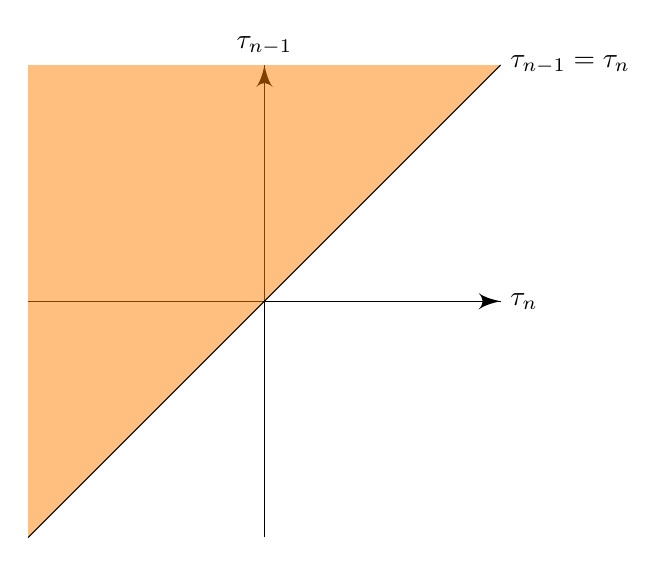
\begin{tikzpicture}
      \draw [->] (-3, 0) -- (3, 0) node [right] {$\tau_n$};
      \draw [->] (0, -3) -- (0, 3) node [above] {$\tau_{n - 1}$};

      \fill [opacity=0.5, morange] (-3, -3) -- (3, 3) -- (-3, 3) -- cycle;
      \draw (-3, -3) -- (3, 3) node [right] {$\tau_{n - 1} = \tau_n$};
    \end{tikzpicture}
  \end{center}
  So we find that
  \[
    S_T = \sum_n (+i)^n \int_{-\infty}^\infty \d \tau_1 \int_{-\infty}^{\tau_1} \d \tau_2 \cdots \int_{-\infty}^{\tau_{n - 1}} V(\tau_n) V(\tau_{n - 1}) \cdots V(\tau_1).
  \]
  We can then see that this is equal to $S^\dagger$.

  What does this tell us? Consider states $\bket{\eta}$ and $\bket{\xi}$ with
  \begin{align*}
    \bket{\eta_T} &= \hat{T} \bket{\eta}\\
    \bket{\xi_T} &= \hat{T} \bket{\xi}
  \end{align*}
  The Dirac bra-ket notation isn't very useful when we have anti-linear operators. So we will write inner products explicitly. We have
  \begin{align*}
    (\eta_T, S\xi_T) &= (\hat{T} \eta, S\hat{T} \xi) \\
    &= (\hat{T} \eta, S_T^\dagger \hat{T} \xi) \\
    &= (\hat{T} \eta, \hat{T} S^\dagger, \xi) \\
    &= (\eta, S^\dagger \xi)^* \\
    &= (\xi, S\eta)
  \end{align*}
  where we used the fact that $\hat{T}$ is anti-unitary. So the conclusion is
  \[
    \brak{\eta_T} S\bket{\xi_T} = \brak{\xi}S\bket{\eta}.
  \]
  So if
  \[
    \hat{T} \mathcal{L}_I(x) \hat{T}^{-1} = \mathcal{L}_I(x_T),
  \]
  then the $S$-matrix elements are equal for time-reversed processes, where the initial and final states are swapped.
\end{eg}

\subsection{CPT theorem}
\begin{thm}[CPT theorem]\index{CPT theorem}
  Any Lorentz invariant Lagrangian with a Hermitian Hamiltonian should be invariant under the product of P, C and T.
\end{thm}
We will not prove this. For details, one can read Streater and Wightman, \emph{PCT, spin and statistics and all that} (1989).

All observations we make suggest that CPT is respected in nature. This means a particle propagating forwards in time cannot be distinguished from the antiparticle propagating backwards in time.

\subsection{Baryogenesis}
In the universe, we observe that there is much more matter than anti-matter. \emph{Baryogenesis}\index{baryogenesis} is the generation of this asymmetry in the universe. Sakarhov came up with three conditions that are necessary for this to happen.
\begin{enumerate}
  \item Baryon number violation (or leptogenesis, ie. lepton number asymmetry), ie. some process $X \to Y + B$ that generates an excess baryon.
  \item Non-equilibrium. Otherwise, the rate of $Y + B \to X$ is the same as the rate of $X \to Y + B$.
  \item C and CP violation. Otherwise, the rate of $X \to Y + B$ and the rate of $\bar{X} \to \bar{Y} + \bar{B}$ would be the same, and the effects cancel out each other.

    We similarly need CP violation, or else the rate of $X \to nq_L$ and the rate of $X \to n q_R$, where $q_{L, R}$ are left and right handed quarks, is equal to the rate of $\bar{x} \to n \bar{q}_L$ and $\bar{x} \to n\bar{q}_R$, and this will wash out our excess.
\end{enumerate}

\section{Spontaneous symmetry breaking}
In this chapter, we are going to look at spontaneous symmetry breaking. The general setting is as follows --- our Lagrangian $\mathcal{L}$ enjoys some symmetry. However, the potential has \emph{multiple} minima. Usually, in perturbation theory, we imagine we are sitting near an equilibrium point of the system (the ``vacuum''), and then look at what happens to small perturbations near the equilibrium.

When there are multiple minima, we have to arbitrarily pick a minimum to be our vacuum, and then do perturbation around it. In many cases, this choice of minimum is \emph{not} invariant under our symmetries. Thus, even though the theory itself is symmetric, the symmetry is lost once we pick a vacuum. It turns out interesting things happen when this happens.

\subsection{Discrete symmetry}
We first consider the case of a discrete symmetry. Consider a real scalar field $\phi(x)$ with a symmetric potential $V(\phi)$, so that
\[
  V(-\phi) = V(\phi).
\]
This gives a discrete ($\Z/2$) symmetry $\phi \leftrightarrow -\phi$.

We will consider the case of a $\phi^4$ theory, with Lagrangian
\[
  \mathcal{L} = \frac{1}{2} \partial_\mu \phi \partial^\mu \phi - \left(\frac{1}{2} m^2 \phi^2 - \frac{\lambda}{4!} \phi^4\right)
\]
for some $\lambda$.

We want the potential to $\to \infty$ as $\phi \to \infty$, so we necessarily require $\lambda > 0$. However, since the $\phi^4$ term dominates for large $\phi$, We are now free to pick the sign of $m^2$, and still get a sensible theory.

Usually, this theory has $m^2 > 0$, and thus $V(\phi)$ has a minimum at $\phi = 0$:
\begin{center}
  \begin{tikzpicture}
    \draw [->](-3, 0) -- (3, 0) node [right] {$\phi$};
    \draw [->] (0, -1.2) -- (0, 3) node [above] {$S(\phi)$};

    \draw [mblue, thick, domain=-1.414:1.414, samples=50] plot [smooth] (\x, {4 * ((\x/2)^4 + (\x/2)^2)});
  \end{tikzpicture}
\end{center}
However, we could imagine a scenario where $m^2 < 0$. In this case, the potential looks like
\begin{center}
  \begin{tikzpicture}
    \draw [->](-3, 0) -- (3, 0) node [right] {$\phi$};
    \draw [->] (0, -1.2) -- (0, 3) node [above] {$V(\phi)$};

    \draw [mblue, thick, domain=-2.4:2.4, samples=50] plot [smooth] (\x, {4 * ((\x/2)^4 - (\x/2)^2)});

    \draw [dashed] (1.414, 0) node [above] {$v$} -- (1.414, -1);
  \end{tikzpicture}
\end{center}
To understand this potential better, we complete the square, and write it as
\[
  V(\phi) = \frac{\lambda}{4} (\phi^2 - v^2)^2 + \text{constant},
\]
where
\[
  v = \sqrt{-\frac{m^2}{\lambda}}.
\]
We see that now $\phi = 0$ become a local maximum, and there are two (global) minima at $\phi = \pm v$. In particular, $\phi$ has acquired a non-zero \term{vacuum expectation value} (\term{VEV}).

We shall wlog consider small excitations around $\phi = v$. Let's write
\[
  \phi(x) = v + cf(x).
\]
Then we can write the Lagrangian as
\[
  \mathcal{L} = \frac{1}{2} \partial_\mu f \partial^\mu f - \lambda \left(v^2 f^2 + + vf^3 + \frac{1}{4} f^4\right),
\]
plus some constants. Therefore $f$ is a scalar field with mass
\[
  m_f^2 = 2v^2 \lambda.
\]
This $\mathcal{L}$ is \emph{not} invariant under $f \to -f$. The symmetry of the original Lagrangian has been broken by the VEV of $\phi$.

\subsection{Continuous symmetry}
We can consider a slight generalization of the above scenario. Consider an $n$-component real scalar field $\phi = (\phi_1, \phi_2, \cdots, \phi_N)^T$, with Lagrangian
\[
  \mathcal{L} = \frac{1}{2} (\partial^\mu \phi) \cdot (\partial_\mu \phi) - V(\phi),
\]
where
\[
  V(\phi) = \frac{1}{2} m^2 \phi^2 + \frac{\lambda}{4} \phi^4.
\]
As before, we will require that $\lambda > 0$.

This is a theory that is invariant under global $\Or(N)$ transforms of $\phi$. Again, if $m^2 > 0$, then $\phi = 0$ is a global minimum, and we do not have spontaneous symmetry breaking. Thus, we consider the case $m^2 < 0$.

In this case, we can write
\[
  V(\phi) = \frac{\lambda}{4} (\phi^2 - v^2)^2 + \text{constant},
\]
where
\[
  v = -\frac{m^2}{\lambda} > 0.
\]
So \emph{any} $\phi$ with $\phi^2 = v^2$ gives a global minimum of the system, and so we have a continuum of vacua. We call this a \term{Sombrero potential} (or \term{wine bottle potential}).
% include sketch

Without loss of generality, we may choose the vacuum to be
\[
  \phi_0 = (0, 0, \cdots, 0, v)^T.
\]
We can then consider steady small fluctuations about this:
\[
  \phi(x) = (\pi_1(x), \pi_2(x), \cdots, \pi_{N-1}(x), v + \sigma(x))^T.
\]
We now have a $\pi$ field with $N - 1$ components, plus a $1$-component $\sigma$ field.

We rewrite the Lagrangian in terms of the $\pi$ and $\sigma$ fields as
\[
  \mathcal{L} = \frac{1}{2}(\partial^\mu \pi) \cdot (\partial_\mu \pi) + \frac{1}{2}(\partial^\mu \sigma) \cdot (\partial_\mu \sigma) - V(\pi, \sigma),
\]
where
\[
  V(\pi, \sigma) = \frac{1}{2} m_\sigma^2 \sigma^s + \lambda v(\sigma^2 + \pi^2) \sigma + \frac{\lambda}{4}(\sigma^2 + \pi^2)^2.
\]
Again, we have dropped a constant term.

In this Lagrangian, we see that the $\sigma$ field has mass
\[
  m_\sigma = \sqrt{2\lambda v^2},
\]
but the $\pi$ fields are massless. We can understand this as follows --- the $\sigma$ field corresponds to the radial direction in the potential, and this is locally quadratic, and hence has a mass term. However, the $\pi$ fields correspond to the excitations in the azimuthal directions, which are flat.

\subsection{General case}
What we just saw is a completely general phenomenon. Suppose we have an $N$-dimensional field $\phi = (\phi_1, \cdots, \phi_N)$, and suppose our theory has a Lie group of symmetries $G$. We will assume that the action of $G$ preserves the potential and kinetic terms individually, and not just the Lagrangian as a whole, so that $G$ will send a vacuum to another vacuum.

Suppose there is more than one choice of vacuum. We write
\[
  \Phi_0 = \{\phi_0: V(\phi_0) = V_{\mathrm{min}}\}
\]
for the set of all vacua. Now we pick a favorite vacuum $\phi_0 \in \Phi_0$, and we want to look at the elements of $G$ that fixes this vacuum. We write
\[
  H = \stab(\phi_0) = \{h \in G: h \phi_0 = \phi_0\}.
\]
This is the \term{invariant subgroup}, or \term{stabilizer subgroup} of $\phi_0$. This is the symmetry we are left with after the spontaneous symmetry breaking.

We will make some further simplifying assumptions. We will suppose $G$ acts \emph{transitively} on $\Phi_0$, ie. given any two vacua $\phi_0, \phi_0'$, we can find some $g \in G$ such that
\[
  \phi_0' = g \phi_0.
\]
This ensures that any two vacua are ``the same'', so which $\phi_0$ we pick doesn't really matter. Indeed, given two such vacua and $g$ relating them, it is a straightforward computation to check that
\[
  \stab(\phi_0') = g \stab(\phi_0) g^{-1}.
\]
So any two choices of vacuum will result in conjugate, and in particular isomorphic, subgroups $H$.

It is a curious, and also unimportant, observation that we given a choice of vacuum $\phi_0$, we have a canonical bijection
\[
  \begin{tikzcd}[cdmap]
    G/H \ar[r, "\sim"] & \Phi_0\\
    g \ar[r, maps to] & g \phi_0
  \end{tikzcd}.
\]
So we can identify $G/H$ and $\Phi_0$.

We now try to understand what happens when we try to do perturbation theory around our choice of vacuum. At $\phi = \phi_0 + \delta \phi$, we can as usual write
\[
  V(\phi_0 + \delta \phi) - V(\phi_0) = \frac{1}{2} \delta \phi_r \frac{\partial^2 V}{\partial \phi_r \partial \phi_s} \delta \phi_s + O(\delta \phi^3).
\]
This quadratic $\partial^2 V$ term is now acting as a mass. We call it the \term{mass matrix}
\[
  M_{rs}^2 = \frac{\partial^2 V}{\partial \phi_r \partial \phi_s}.
\]
Note that we are being sloppy with where our indices go, because $(M^2)^{rs}$ is ugly. It doesn't really matter much, since $\phi$ takes values in $\R^N$ (or $\C^n$), which is a Euclidean space.

In our previous example, we saw that there were certain modes that went massless. We now want to see if the same happens. To do so, we pick a basis $\{\tilde{t}^a\}$ of $\mathfrak{h}$ (the Lie algebra of $H$), and then extend it to a basis $\{t^a, \theta^a\}$ of $\mathfrak{g}$.

We consider a variation
\[
  \delta \phi = \varepsilon \theta^a \phi_0
\]
around $\phi_0$.

Note that when we write $\theta^a \phi_0$, we mean the resulting infinitesimal change of $\phi_0$ when $\theta^a$ acts on field. For a general Lie algebra element, this may be zero. However, we know that $\theta^a$ does not belong to $\mathfrak{h}$, so it does not fix $\phi_0$. Thus (assuming sensible non-degeneracy conditions) this implies that $\theta^a \phi_0$ is non-zero.

At this point, the uncareful reader might be tempted to say that since $G$ is a symmetry of $V$, we must have $V(\phi_0 + \delta \phi) = V(\phi_0)$, and thus
\[
  (\theta^a \phi)_r M_{rs}^2 (\theta^a \phi)_s = 0,
\]
and so we have found zero eigenvectors of $M_{rs}$. But this is wrong. For example, if we take
\[
  M =
  \begin{pmatrix}
    1 & 0\\
    0 & -1
  \end{pmatrix},\quad
  \theta^a \phi =
  \begin{pmatrix}
    1\\1
  \end{pmatrix},
\]
then our previous equation holds, but $\theta^a \phi$ is \emph{not} a zero eigenvector. We need to be a bit more careful.

Instead, we note that by definition of $G$-invariance, for any field value $\phi$ and a corresponding variation
\[
  \phi \mapsto \phi + \varepsilon \theta^a \phi,
\]
we must have
\[
  V(\phi + \delta \phi) = V(\phi),
\]
since this is what it means for $G$ to be a symmetry.

Expanding to first order, this says
\[
  V(\phi + \delta \phi) - V(\phi) = \varepsilon (\theta^a \phi)_r \frac{\partial V}{\partial \phi_r} = 0.
\]
Now the trick is to take a further derivative of this. We obtain
\[
  0 = \frac{\partial}{\partial \phi_s} \left((\theta^a \phi)_r \frac{\partial V}{\partial \phi_r}\right) = \left(\frac{\partial}{\partial \phi_s} (\theta^a \phi)_r\right) \frac{\partial V}{\partial \phi_r} + (\theta^a \phi)_r M_{rs}^2.
\]
Now at a vacuum $\phi = \phi_0$, the first term vanishes. So we must have
\[
  (\theta^a \phi_0)_r M_{rs}^2 = 0.
\]
By assumption, $\theta^a \phi_0 \not= 0$. So we have found a zero vector of $M_{rs}$. Recall that we had $\dim G - \dim H$ of these $\theta^a$ in total. So we have found $\dim G - \dim H$ zero eigenvectors in total.

We can do a small sanity check. What if we replaced $\theta^a$ with $t^a$? The same derivations would still follow through, and we deduce that
\[
  (t^a \phi_0)_r M_{rs}^2 = 0.
\]
But since $t^a$ is an \emph{unbroken symmetry}, we actually just have $t^a \phi_0 = 0$, and this really doesn't say anything interesting.

What about the other eigenvalues? They could be zero for some other reason, and there is no reason to believe one way or the other. However, generally, in the scenarios we meet, they are usually massive. So after spontaneous symmetry breaking, we end up with $\dim G - \dim H$ massless modes, and $N - (\dim G - \dim H)$ massive ones.

This is \term{Goldstone's theorem} in the classical case.
\begin{eg}
  In our previous $O(N)$ model, we had $G = O(N)$, and $H = O(N - 1)$. These have dimensions
  \[
    \dim G = \frac{N(N - 1)}{2},\quad \dim H = \frac{(N - 1)(N - 2)}{2}.
  \]
  Then we have
  \[
    \Phi_0 \cong S^{N - 1},
  \]
  the $(N - 1)$-dimensional sphere. So we expect to have
  \[
    \frac{N - 1}{2} (N - (N - 2)) = N - 1
  \]
  massless modes, which are the $\pi$ fields we found. We also found $N - (N - 1) = 1$ massive mode, namely the $\sigma$ field.
\end{eg}

\begin{eg}
  In the first discrete case, we had $G = \Z/2\Z$ and $H = \{e\}$. These are (rather degenerate) $0$-dimensional Lie groups. So we expect $0 - 0 = 0$ massless modes, and $1 - 0 = 1$ massive modes, which is what we found.
\end{eg}
\subsection{Goldstone's theorem}
We now consider the quantum version of Goldstone's theorem. We hope to get something similar.

Again, suppose our Lagrangian has a symmetry group $G$, which is spontaneously broken into $H \leq G$ after picking a preferred vacuum $\bket{0}$. Again, we take a Lie algebra basis $\{t_a, \theta_a\}$ of $\mathfrak{g}$, where $\{t_a\}$ is a basis for $\mathfrak{h}$. Note that we will assume that $a$ runs from $1, \cdots, \dim G$, and we use the first $\dim H$ labels to refer to the $t_a$, and the remaining to label the $\theta_a$, so that the actual basis is
\[
  \{t_1, t_2, \cdots, t_{\dim H}, \theta_{\dim H + 1}, \cdots, \theta_{\dim G}\}.
\]
For aesthetic reasons, this time we put the indices on the generators below.

Now recall, say from AQFT, that these symmetries of the Lagrangian give rise to conserved currents $j_a^\mu(x)$. These in turn give us conserved charges
\[
  Q_a = \int \d^3 x\; j^0_a (x).
\]
Moreover, under the action of the $t^a$ and $\theta^a$, the corresponding change in $\phi$ is given by
\[
  \delta \phi = -[Q^a, \phi].
\]
The fact that the $\theta^a$ break the symmetry of $\brak{0}$ tell us that
\[
  \brak{0}[Q^a, \phi(0)] \bket{0} \not= 0.
\]
Note that the choice of evaluating $\phi$ at $0$ is completely arbitrary, but we have to pick somewhere, and $0$ is easy to write. Writing out the definition of $Q_a$, we know that
\[
  \int \d^3 x\; \brak{0} [j_a^0(x), \phi(0)] \bket{0} \not= 0.
\]
More generally, since the label $^0$ is arbitrary by Lorentz invariance, we are really looking at the relation
\[
  \brak{0} [j_a^\mu (x), \phi(0)] \bket{0} \not= 0,
\]
and writing it in this more Lorentz covariant way makes it easier to work with. The goal is to deduce the existence of massless states from this non-vanishing.

For convenience, we will write this expression as
\[
  X_a^\mu = \brak{0} [j_a^\mu (x), \phi(0)] \bket{0}.
\]
We treat the two terms in the commutator separately. The first term is
\[
  \brak{0} j_a^\mu (x) \phi(0) \bket{0} = \sum_n \brak{0}j_a^\mu (x) \bket{n} \brak{n}\phi(0) \bket{0}.\tag{$*$}
\]
We write $p_n$ for the momentum of $\bket{n}$. We now note that
\[
  j_a^\mu (x) = e^{i\hat{p} \cdot x} j_a^\mu (0) e^{-i\hat{p} \cdot x}.
\]
so that
\[
  \brak{0}j_a^\mu(x) \bket{n} = \brak{0} j_a^\mu(0) \bket{n} e^{-ip_n \cdot x}.
\]
We can use this to do some Fourier transform magic. By direct verification, we can see that $(*)$ is equivalent to
\[
  i \int \frac{\d^4 k}{(2\pi)^3} \rho_a^\mu(k) e^{-ik\cdot x},
\]
where
\[
  i \rho_a^\mu (k) = (2\pi)^3 \sum_n \delta^4(k - p_n)\brak{0}j_a^\mu(0) \bket{n} \brak{n}\phi(0)\bket{0}.
\]
Similarly, we define
\[
  i \tilde{\rho}_a^\mu (k) = (2\pi)^3 \sum_n \delta^4(k - p_n) \brak{0} \phi(0) \bket{n} \brak{n} j_a^\mu (0) \bket{0}.
\]
Then we can write
\[
  X_a^\mu = i \int \frac{\d^4 k}{(2\pi)^3}\left(\rho_a^\mu (k) e^{-ik\cdot x} - \tilde{\rho}_a^\mu(k) e^{+ik\cdot x}\right).
\]
This is called the \term{K\"allen-Lehmann spectral representation}.

We now claim that $\rho_a^\mu(k)$ and $\tilde{\rho}_a^\mu(k)$ can be written in a particularly nice form. This involves a few observations (when I say $\rho_a^\mu$, I actually mean $\rho_a^\mu$ and $\tilde{\rho}_a^\mu$):
\begin{itemize}
  \item $\rho_a^\mu$ depends Lorentz covariantly in $k$. So it ``must'' be a scalar multiple of $k^\mu$.
  \item $\rho_a^\mu(k)$ must vanish when $k^0 > 0$, since $k^0 \leq 0$ is non-physical. % why?
  \item By Lorentz invariance, the magnitude of $\rho_a^\mu(k)$ can depend only on the length (squared) $k^2$ of $k$.
\end{itemize}
Under these assumptions, we can write can write $\rho_a^\mu$ and $\tilde{\rho}_a^\mu$ as
\begin{align*}
  \rho_a^\mu (k) &= k^\mu \Theta(k^0) \rho_a (k^2),\\
  \tilde{\rho}_a^\mu (k) &= k^\mu \Theta(k^0) \tilde{\rho}_a(k^2),
\end{align*}
where $\Theta$ is the \term{Heaviside theta function}
\[
  \Theta(x) =
  \begin{cases}
    1 & x > 0\\
    0 & x \leq 0
  \end{cases}.
\]
So we can write
\[
  X_a^\mu = i \int \frac{\d^4 k}{(2\pi)^3}\;k^\mu \Theta(k^0) (\rho_a(k^2)e^{-ik\cdot x} - \tilde{\rho}_a(k^2) e^{+ik\cdot x}).
\]
We now use the (nasty?) trick of hiding the $k^\mu$ by replacing it with a derivative:
\[
  X_a^\mu = - \partial^\mu \int \frac{\d^4 k}{(2\pi)^3} \Theta(k^0)\left(\rho_a(k^2) e^{-ik\cdot x} + \tilde{\rho}_a(k^2) e^{ik\cdot x}\right).
\]
Now we might find the expression inside the integral a bit familiar. Recall that the propagator is given by
\[
  D(x, \sigma) = \brak{0} \phi(x) \phi(0) \bket{0} = \int \frac{\d^4 k}{(2\pi)^3}\; \Theta(k^0) \delta(k^2 - \sigma) e^{-ik\cdot x}.
\]
where $\sigma$ is the square of the mass of the field. Using the really silly fact that
\[
  \rho_a(k^2) = \int \d \sigma\; \rho_a(\sigma) \delta(k^2 - \sigma),
\]
we find that
\[
  X_a^\mu = -\partial^\mu \int \d \sigma\; (\rho_a(\sigma) D(x, \sigma) + \tilde{\rho}_a (\sigma) D(-x, \sigma)).
\]
Now we have to recall more properties of $D$. For spacelike $x$, we have $D(x, \sigma) = D(-x, \sigma)$. Therefore, requiring $X_a^\mu$ to vanish for spacelike $x$ by causality, we see that we must have
\[
  \rho_a(\sigma) = - \tilde{\rho}_a(\sigma).
\]
Therefore we can write
\[
  X_a^\mu = -\partial^\mu \int \d \sigma\; \rho^a(\sigma) i\Delta(x, \sigma),\tag{$\dagger$}
\]
where
\[
  i \Delta(x, \sigma) = D(x, \sigma) - D(-x, \sigma) = \int \frac{\d^4 k}{(2\pi)^3} \delta(k^2 - \sigma) \varepsilon(k^0) e^{-ik\cdot x},
\]
and
\[
  \varepsilon(k^0) =
  \begin{cases}
    +1 & k^0 > 0\\
    -1 & k^0 < 0
  \end{cases}.
\]
This $\Delta$ is again a different sort of propagator.

We now use current conservation, which tells us
\[
  \partial_\mu j^\mu_a = 0.
\]
So we must have
\[
  \partial_\mu X_a^\mu =- \partial^2 \int \d \sigma\; \rho_a(\sigma) i \Delta(x, \sigma) = 0.
\]
On the other hand, by inspection, we see that $\Delta$ satisfies the Klein-Gordon equation
\[
  (\partial^2 + \sigma) \Delta = 0.
\]
So in $(\dagger)$, we can replace $-\partial^2 \Delta$ with $\sigma \Delta$. So we find that
\[
  \partial_\mu X_a^\mu = \int \d \sigma\; \sigma \rho^a (\sigma) i \Delta(x, \sigma) = 0.
\]
This is true for all $x$. In particular, it is true for timelike $x$ where $\Delta$ is non-zero. So we must have
\[
  \sigma \rho_a(\sigma) = 0.
\]
But we also know that $\rho_a(\sigma)$ cannot be identically zero, because $X_a^\mu$ is not. So the only possible explanation is that
\[
  \rho_a(\sigma) = N_a \delta(\sigma),
\]
where $N_a$ is a dimensionful non-zero constant.

Now we retrieve our definitions of $\rho_a$. Recall that they are defined by
\begin{align*}
  i \rho_a^\mu (k) &= (2\pi)^3 \sum_n \delta^4(k - p_n)\brak{0}j_a^\mu(0) \bket{n} \brak{n}\phi(0)\bket{0}\\
  \rho_a^\mu (k) &= k^\mu \Theta(k^0) \rho_a (k^2).
\end{align*}
So the fact that $\rho_a(\sigma) = N_a \delta(\sigma)$ implies that there must be some states, which we shall call $\bket{B(p)}$, of momentum $p$, such that $p^2 = 0$, and
\begin{align*}
  \brak{0}j_a^\mu(0)\bket{B(p)} &\not= 0\\
  \brak{B(p)} \phi(0) \bket{0} &\not= 0.
\end{align*}
The condition that $p^2 = 0$ tell us these particles are massless, which are those massless modes we were looking for! These are the \term{Goldstone bosons}.

We can write the values of the above as
\begin{align*}
  \brak{0} j_a^\mu (0)\bket{B(p)} &= i F_a^B p^\mu\\
  \brak{B(p)} \phi(0)\bket{0} &= Z^B,
\end{align*}
whose form we deduced by Lorentz in/covariance. By dimensional analysis, we know $F_{aB}$ is a dimension $-1$ constant, and $Z_B$ is a dimensionless constant.

From these formulas, we note that since $\phi(0)\bket{0}$ is rotationally invariant, we deduce that $\bket{B(p)}$ also is. So we deduce that these are in fact spin $0$ particles.

Finally, we end with some computations that relate these different numbers we obtained. We will leave the computational details for the reader, and just outline what we should do. Using our formula for $\rho$, we find that
\[
  \brak{0} [j_a^\mu(x), \phi(0)] \bket{0} = - \partial^\mu \int N^a \delta (\sigma) i \Delta(x, \sigma) \;\d \sigma = -iN^a \partial^\mu \Delta(x, 0).
\]
Integrating over space, we find
\[
  \brak{0}[Q_a, \phi(0)]\bket{0} = - iN_a \int \d^3 x\; \partial^0 \Delta(x, 0) = i N_a.
\]
Then we have
\[
  \brak{0} t_a \phi(0)\bket{0} = i \brak{0} [Q_a, \phi(0)]\bket{0} = i \cdot i N_a = -N_a.
\]
So this number $N_a$ sort-of measures how much the symmetry is broken, and we once again see that it is the breaking of symmetry that gives rise to a non-zero $N_a$, hence the massless bosons.

We also recall that we had
\[
  i k^\mu \Theta(k^0) N_a \delta(k^2) = \sum_B \int \frac{\d^3 p}{2|\mathbf{p}|}\; \delta^4(k - p) \brak{0} j_a^\mu(0) \bket{B(p)} \brak{B(p)} \phi(0) \bket{0}.
\]
On the RHS, we can plug in the names we gave for the matrix elements, and on the left, we can write it as an integral
\[
  \int \frac{\d^3 p}{2|\mathbf{p}|} \delta^4 (k - p) i k^\mu N_a = \int \frac{\d^3 p}{2|\mathbf{p}|} \delta^4(k - p) i p^\mu \sum_B F_a^B Z^B.
\]
So we must have
\[
  N^a = \sum_B F_a^B Z^B.
\]
Now for each independent symmetry-breaking $\theta^a \in \mathfrak{g} \setminus \mathfrak{h}$, we obtain a Goldstone boson this way. So all together, we find
\[
  n = \dim G - \dim H
\]
many Goldstone bosons.

%The number of broken generators is
%\[
% n = \dim G - \dim H.
%\]
%So we see that there are $n$ of the $\rho^a$ that have non-zero contributions at $\sigma = 0$.
%
%Here $F_{aB}$ is a rank $n$ matrix, and this gives rise to $n$ Goldstone bosons $B$.

It is important to figure out the assumptions we used to derive the result. We mentioned ``Lorentz invariance'' many times in the proof, so we certainly need to assume our theory is Lorentz invariant. While it may not seem obvious, the proof actually requires there are more than $2$ spacetime dimensions, and in fact the result does not hold in $2$ or $1$ dimensions. Another perhaps subtle point is that we also needed states to have a positive definite norm. % revisit

It turns out in the case of gauge theory, these do not necessarily hold, and we need to work with them separately.

%Note that we assumed we have a Lorentz invariant theory, and we also assumed there were more than $2$ spacetime dimensions. We don't get spontaneous symmetry breaking in $2$ or $1$ dimensions. We also assumed that states have a positive definite norm. % something about things cancelling.


%We now consider spontaneous symmetry breaking in a fully quantum way. Again, the symmetry group $G$ of the Lagrangian is broken spontaneously to $H \leq G$. In other words, the scalar field gets a non-zero vacuum expectation value
%\[
% \brak{0} \phi(x) \bket{0} = \phi_0 \not= 0.
%\]
%The VEV is invariant under $h \in H$, and so
%\[
% \brak{0} h \phi(x) \bket{0} = \phi_0,
%\]
%but this is not invariant under a general $g \in G \setminus H$. Again suppose we have a basis
%\[
% t^a = \{\tilde{t}^i, \tilde{\theta}^{\tilde{a}}\}
%\]
%of $\mathfrak{g}$, where $\tilde{t}^i$ span $\mathfrak{h} \leq \mathfrak{g}$.
%
%Since $G$ is a symmetry of the Lagrangian, we know there are conserved currents and charges, say $j_a^\mu (x)$ and
%\[
% Q_a = \int \d^3 x\; j^0_a = \int \d^3 x\; \pi(x) t_a \phi,
%\]
%where $\pi$ is the conjugate field. Using the canonical commutation relations, we have
%\[
% \delta \phi(0) = i \alpha^a t^a \phi(0) = - [Q^a, \phi(0)] \alpha^a.
%\]
%Thus these charges induce a representation on the Lie algebra of $\phi$. % ???
%
%To investigate excitations from spontaneous symmetry breaking, consider the VEV of
%\[
% X_a^\mu = \brak{0}[j_a^\mu (x), \phi(0)]\bket{0} = \sum_n \left( \brak{0}j_a^\mu (x) \bket{n} \brak{n}\phi(0) \bket{0} - \brak{0}\phi(0) \bket{n} \brak{n}j_a^\mu(x) \bket{0}\right).
%\]
%We can then write this as
%\[
% i \int \frac{\d^4 k}{(2\pi)^3}\left(\rho_a^\mu (k) e^{-ik\cdot x} - \tilde{\rho}_a^\mu(k) e^{+ik\cdot x}\right),
%\]
%where
%\begin{align*}
% i \rho_a^\mu (k) &= (2\pi)^3 \sum_n \delta^4(k - p_n)\brak{0}j_a^\mu(0) \bket{n} \brak{n}\phi(0)\bket{0}\\
% i \tilde{\rho}_a^\mu (k) &= (2\pi)^3 \sum_n \delta^4(k - p_n) \brak{0} \phi(0) \bket{n} \brak{n} j_a^\mu (0) \bket{0}
%\end{align*}
%Note that we had $j_a^\mu(0)$ because the $e^{-ik\cdot x}$ factors generated the translations. Here $p_n$ is the $4$-momentum of $n$. % ???
%This is called the \term{K\"allen-Lehmann spectral representation}.
%
%From the Lorentz covariance of $\rho_a^\mu$ and $\tilde{\rho}_a^\mu$, they must be proportional to $k^\mu$, as that is the only $4$-vector we have that they can be proportional to. % huh?
%
%Physical states have $k^0 > 0$. Then we can write
%\[
% \rho_a^\mu (k) = k^\mu \Theta(k^0) \rho_a (k^2), % This is k squared.
%\]
%where $\Theta$ is the Heaviside function. Similarly, we have
%\[
% \tilde{\rho}_a^\mu (k) = k^\mu \Theta(k^0) \tilde{\rho}_a(k^2).
%\]
%Then we have
%\[
% X_a^\mu = - \partial^\mu \int \frac{\d^4 k}{(2\pi)^3} \Theta(k^0)\left(\rho_a(k^2) e^{-ik\cdot x} + \tilde{\rho}_a(k^2) e^{ik\cdot x}\right).
%\]
%We can try to relate this to the propagator,
%\[
% D(z - y, \sigma) = \brak{0} \phi(x) \phi(y) \bket{0}, % should be phi(z)
%\]
%where $\sigma$ is the square of the mass of the field. We can write this as
%\[
% D(z - y, \sigma) = \int \frac{\d^4 p}{(2\pi)^3} \Theta(p^0) \delta(p^4 - \sigma) e^{-ip\cdot (z - y)}. % what is p^4?
%\]
%Then we can write
%\[
% X_a^\mu = -\partial_\mu \int \d \sigma (\rho_a(\sigma) D(x, \sigma) + \tilde{\rho}_a (\sigma) D(-x, \sigma)).
%\]
%Here we used the fact that
%\[
% \rho(k^2) = \int \d \sigma\; \rho(\sigma) \delta(k^2 - \sigma).
%\]
%Now for spacelike $x$, we have $D(x, \sigma) = D(-x, \sigma)$. Therefore, requiring $X_a^\mu$ to vanish for spacelike $x$ by causality, we see that
%\[
% \rho_a(\sigma) = - \tilde{\rho}_a(\sigma).
%\]
%Therefore we can write
%\[
% X_a^\mu = -\partial^\mu \int \d \sigma\; \rho^a(\sigma) i\Delta(x, \sigma),\tag{$\dagger$}
%\]
%where
%\[
% i \Delta(x, \sigma) = D(x, \sigma) - D(-x, \sigma) = \int \frac{\d^4 k}{(2\pi)^3} \delta(k^2 - \sigma) \varepsilon(k^0) e^{-ik\cdot x},
%\]
%where
%\[
% \varepsilon(k^0) =
% \begin{cases}
% +1 & k^0 > 0\\
% -1 & k^0 < 0
% \end{cases}.
%\]
%We can think of this as some different sort of propagator. For spacelike $x$, this vanishes.
%
%We now use current conservation, so
%\[
% \partial_\mu j^\mu_a = 0.
%\]
%So we find
%\[
% \partial_\mu X_a^\mu =- \partial^2 \int \d \sigma\; \rho_a(\sigma) i \Delta(x, \sigma) = 0.
%\]
%Also, the Klein-Gordon equation gives
%\[
% (\partial^2 + \sigma) \Delta = 0.
%\]
%So we can replace $-\partial^s \Delta$ with $\sigma \Delta$. So
%\[
% \partial_\mu X_a^\mu = \int \d \sigma\; \sigma \rho^a (\sigma) i \Delta(x, \sigma) = 0.
%\]
%This is true for all $x$. In particular, it is true for timelike $x$ where $\Delta$ is non-zero. So we need
%\[
% \sigma \rho(\sigma) = 0.
%\]
%There are two possibilities:
%\begin{enumerate}
% \item $\rho(\sigma) = 0$. This means
% \[
% \brak{0} [j_a^\mu(x), \phi(0)] \bket{0} = 0.
% \]
% So $t^a$ is an unbroken symmetry, and
% \[
% \brak{0} t^a \phi\bket{0} = 0.
% \]
% \item $\rho^a(\sigma) = N^a \delta(\sigma)$, where $N^a$ is a dimensionful non-zero constant.
%\end{enumerate}
%The first case is boring, so we want to figure out what the consequences of (ii) are. Plugging this into $(\dagger)$, we get
%\[
% \brak{0} [j_a^\mu(x), \phi(0)] \bket{0} = - \partial^\mu \int N^a \delta (\sigma) i \Delta(x, \sigma) \;\d \sigma = -iN^a \partial^\mu \Delta(x, 0).
%\]
%Integrating over time, we find
%\[
% \brak{0}[Q^a, \phi(0)]\bket{0} = - iM^a \int \d^3 x\; \partial^0 \Delta(x, 0) = i N^a.
%\]
%Then we have\[
% \brak{0} t^a \phi_0\bket{0} = i \brak{0} [Q^a, \phi(0)]\bket{0} = i \cdot i N^a = -N^a.
%\]
%Now if $N^a$ and $\phi_0$ are both non-zero, then some states in $\rho_a^\mu$ and $\tilde{\rho}_a^\mu$ have non-zero matrix elements. Label these states by $B(p)$. From Lorentz covariance and dimensional analysis, we have
%\begin{align*}
% \brak{0} j_a^\mu (0)\bket{B(p)} &= i F_{aB} p^\mu\\
% \brak{B(p)} \phi(0)\bket{0} &= Z_B,
%\end{align*}
%where $F_{aB}$ is a dimension $-1$ constant, and $Z_B$ is a dimensionless constnat.
%
%We see that $B(p)$ are spin zero by rotation invariance, and massless (only contribute when $\sigma = p^2 = 0$). We have
%\[
% i \rho_a^\mu (k) = i k^\mu \Theta(k^0) N^a \sigma(k^2) = \sum_B \int \frac{\d^3 p}{2|\mathbf{p}|} \delta^4(k - p) \brak{0} j_a^\mu(0) \bket{B(p)} \brak{B(p)} \phi(0) \bket{0}.
%\]
%We write the LHS as an integral, and plug in the matrix element on the RHS. Then we see that
%\[
% \int \frac{\d^3 p}{2|\mathbf{p}|} \delta^4 (k - p) i k^\mu N^a = \int \frac{\d^3 p}{2|\mathbf{p}|} \delta^4(k - p) i p^\mu \sum_B F_{aB} Z_B.
%\]
%So we have
%\[
% N^a = \sum_B F_{aB} Z_B.
%\]
%The number of broken generators is
%\[
% n = \dim G - \dim H.
%\]
%So we see that there are $n$ of the $\rho^a$ that have non-zero contributions at $\sigma = 0$.
%
%Here $F_{aB}$ is a rank $n$ matrix, and this gives rise to $n$ Goldstone bosons $B$.
%
%Note that we assumed we have a Lorentz invariant theory, and we also assumed there were more than $2$ spacetime dimensions. We don't get spontaneous symmetry breaking in $2$ or $1$ dimensions. We also assumed that states have a positive definite norm. % something about things cancelling.

\subsection*{The Higgs mechanism}
The Higgs mechanism is spontaneous symmetry breaking in a gauge theory. The above proof required the states to have positive definite norm, and gauge theory doesn't satisfy this property.

For example, in QED, imposing a Lorentz invariant gauge condition (eg. the Lorentz gauge) gives us negative norm states. On the other hand, if we fix the gauge condition so that we don't have negative norm states, this breaks Lorentz invariance.

As a first step to see what happens in this case, let's first consider scalar electrodynamics with a complex scalar field $\phi(x)$ and photon $A_\mu(x)$. As usual, the Lagrangian is
\[
  \mathcal{L} = -\frac{1}{4} F_{\mu\nu} F^{\mu\nu} + (\D_\mu \phi)^* (\D^\mu \phi) - V(|\phi|^2).
\]
It is useful to recap that under a $\U(1)$ gauge transformation, given by $\alpha(x) \in \R$, the fields transform as
\begin{align*}
  \phi(x) &\mapsto e^{i\alpha(x)} \phi(x)\\
  A_\mu(x) &\mapsto A_\mu(x) - \frac{1}{q} \partial_\mu \alpha(x).
\end{align*}
We will consider a $\phi^4$ theory, so that the potential is
\[
  V(|\phi|^2) = \mu^2 |\phi|^2 + \lambda |\phi|^4,
\]
where $\lambda > 0$.

This is similar to what we have encountered already, but now we have a gauge field. If $\mu^2 > 0$, then $|\phi|^2$ is the usual mass term, with a unique vacuum when $\phi = 0$, and symmetry is preserved. So we have massless $A_\mu$ and a massive $\phi$.

If instead $\mu^2 < 0$, then this is the interesting case. We have a minima at
\[
  |\phi_0|^2 = -\frac{\mu^2}{2\lambda} \equiv \frac{v^2}{2}.
\]
Without loss of generality, we expand around a real $\phi_0$, and write
\[
  \phi(x) = \frac{1}{\sqrt{2}} e^{i \theta(x)/v} (v + \eta(x)),
\]
where $\eta, \theta$ are \emph{real} fields. For small fluctuations, we approximate
\[
  \phi(x) \approx \frac{1}{\sqrt{2}} (v + \eta + i \theta).
\]
We will chose $v > 0$. We substitute this into the potential to get
\[
  V(\phi^* \phi) = \lambda \left(|\phi|^2 - \frac{v^2}{2}\right)^2 = \frac{\lambda}{4} (v^2 + \eta^2 + \theta^2 + 2 v \eta - v^2)^2 % how can we possibly have a $\theta$ field?
\]
where we as usual dropped a constant. Putting this to the Lagrangian, we get
\[
  \mathcal{L} = \frac{1}{2} \left(\partial_\mu \eta \partial^\mu \eta + 2 \mu^2 \eta^2\right) + \frac{1}{2} \partial_\mu \theta \partial^\mu \theta - \frac{1}{4} F^{\mu\nu} F_{\mu\nu} + qv A_\mu \partial^\mu \theta + \frac{q^2 v^2}{2} A_\mu A^\mu + \mathcal{L}_{\mathrm{int}},
\]
where $\mathcal{L}_{\mathrm{int}}$ involves terms with $\geq 2$ fields.

It appears that that we have a mass for $\eta$ and $A_\mu$, but not $\theta$, and also a strange $A_\mu \partial^\mu \theta$ term.

To see what is going on, we transform to the \term{unitary gauge}.
\[
  A_\mu \mapsto A_\mu + \frac{1}{qv} \partial_\mu \theta(x),
\]
where we have chosen
\[
  \alpha(x) = - \frac{1}{v} \theta(x).
\]
Then the $\phi$ field transforms as
\[
  \phi \mapsto e^{i\theta/v} \phi = \frac{1}{2} (v + \eta).
\]
This corresponds to getting rid of the phase, and so we may assume $\phi$ is real. In this gauge, we have
\[
  \mathcal{L} = \frac{1}{2}(\partial^\mu \eta \partial_\mu \eta + 2 \mu^2 \eta^2) - \frac{1}{4} F^{\mu\nu}F_{\mu\nu} + \frac{q^2 v^2}{2} A_\mu A^\mu + \mathcal{L}_{\mathrm{int}}.
\]
We can now just read off what is going on in here.
\begin{itemize}
  \item We have a massive $\eta$ field with mass
    \[
      m_\mu^2 = - 2 \mu^2 = 2 \lambda v^2 > 0.
    \]
  \item The photon has mass
    \[
      m_A^2 = q^2 v^2.
    \]
  \item What would be the Goldstone boson, namely the $\theta$ field has been ``eaten'' to become the longitudinal polarization of $A_\mu$ and $A_\mu$ has gained a degree of freedom.
\end{itemize}
One can check that the interaction piece becomes
\[
  \mathcal{L}_{\mathrm{int}} = \frac{q^2}{2} A^\mu A^\mu \eta^2 + q m_A A_\mu A^\mu \eta - \frac{\lambda}{4} \eta^4 - m_\eta \sqrt{\frac{\lambda}{2}} \eta^3.
\]
So we have interactions that look like
\begin{center}
  \begin{tikzpicture}
    \begin{feynman}
      \vertex (tl);
      \vertex [below right=of tl] (c);
      \vertex [above right=of c] (tr);
      \vertex [below left=of c] (bl);
      \vertex [below right=of c] (br);

      \diagram*{
        (tl) -- [photon] (c) -- [photon] (tr)
        (bl) -- [scalar] (c) -- [scalar] (br)
      };
    \end{feynman}
  \end{tikzpicture}
  \quad
  \begin{tikzpicture}
    \begin{feynman}
      \vertex (tl);
      \vertex [below right=of tl] (c);
      \vertex [above right=of c] (tr);
      \vertex [below =of c] (b);

      \diagram*{
        (tl) -- [photon] (c) -- [photon] (tr)
        (b) -- [scalar] (c);
      };
    \end{feynman}
  \end{tikzpicture}
  \quad
  \begin{tikzpicture}
    \begin{feynman}
      \vertex (tl);
      \vertex [below right=of tl] (c);
      \vertex [above right=of c] (tr);
      \vertex [below left=of c] (bl);
      \vertex [below right=of c] (br);

      \diagram*{
        (tl) -- [scalar] (c) -- [scalar] (tr)
        (bl) -- [scalar] (c) -- [scalar] (br)
      };
    \end{feynman}
  \end{tikzpicture}
  \quad
  \begin{tikzpicture}
    \begin{feynman}
      \vertex (tl);
      \vertex [below right=of tl] (c);
      \vertex [above right=of c] (tr);
      \vertex [below =of c] (b);

      \diagram*{
        (tl) -- [scalar] (c) -- [scalar] (tr)
        (b) -- [scalar] (c);
      };
    \end{feynman}
  \end{tikzpicture}
\end{center}
This $\eta$ field is the ``Higgs boson'' in our toy theory.

\subsection{Non-abelian theories}
That was an abelian gauge theory. What about non-abelian gauge theories?

Let $\psi(x) = (\psi_1(x), \cdots(x), \psi_n(x)) \in \C^n$ be a complex field. % really? % gauge group is a subgroup of unitary group? I think he means there is some gauge group with a unitary representation on \C^n.

We first review the various notations and terminology. A non-abelian gauge transformation is in general of the form
\[
  \psi_i(x) \mapsto U_{ij}(x) \psi_j(x) = \exp(i t^a \theta^a(x)) \psi_j(x),
\]
where $U_{ij}(x) \in \U(n)$ for an $n$-dimensional representation of the unitary group; the $t^a$ are fixed Hermitian generators of $\uu(n)$ and $\theta^a(x)$ are real coefficients. The transformation of $\bar\psi$ is
\[
  \bar\psi(x) \mapsto \bar\psi_j (x) \exp(-i t^a \theta^a(x)).
\]
We suppose the $t^a$ satisfy the relations
\[
  [t^a, t^b] = f^{abc} t^c,
\]
where $f^{abc}$ are the \term{structure constants}. We further suppose we normalize the basis vector so that
\[
  \Tr (t^a t^b) = T(R) \delta^{ab},
\]
and $T(R)$ is the \term{Dynkin index} of the representation $R$, which is $\frac{1}{2}$ for the fundamental representation, which is $\frac{1}{2}$ for the fundamental representation. In the standard model, fermions live in the fundamental or trivial representations of various gauge theories.

We have a covariant derivative given by
\[
  (D_\mu)_{ij} = \partial_\mu \delta_{ij} + i g(t^a A_\mu^a) _{ij}.
\]
We define $F_{\mu\nu}^a$ by
\[
  [D_\mu, D_\nu] = i g t^a F^a_{\mu\nu}.
\]
We can alternatively write it as
\[
  F_{\mu\nu}^a = \partial_\mu A_\nu^a - \partial_\nu A_\mu^a - g f^{abc} A_\mu^b A^c_\nu.
\]
The gauge part of $\mathcal{L}$ is
\[
  \mathcal{L}_g = \frac{1}{4} F_{\mu\nu}^a F^{a\mu\nu} = - \frac{1}{2} \Tr (F_{\mu\nu} F^{\mu\nu}).
\]
In the next chapter, we'll discuss electroweak theory, where we break $\SU(2)_L \times \U(1)_Y$ into $\U(1)_{EM}$. On the second example sheet, we will study cases where we have a breaking from $\SU(2)$ to $\U(1)$, and cases where the scalar transforms in different representations.

\section{Electroweak theory}
In electroweak theory, we have an $\SU(2)_L \times \U(1)_Y$ gauge group. We will not justify this choice, because the only real reason is that it matches experiments well.
\subsection{Electroweak gauge theory}
Here we are going to study the gauge and Higgs part of the theory. As mentioned, the gauge group is $\SU(2)_L \times \U(1)_Y$. We will see that this is broken by the Higgs mechanism. We should have some idea of how things are going to work out based on what we saw in the abelian case.

We have a complex scalar (Higgs) field $\phi(x) \in \C^2$, which is in the doublet (fundamental) representation of $\SU(2)$, and the hypercharge is $Y = \frac{1}{2}$. So under a gauge transformation, the field transforms as
\[
  \phi(x) \mapsto e^{i \alpha^(x) \tau^a} e^{i \beta(x) \frac{1}{2}} \phi(x),
\]
where the $\tau^a$ are the generators given by
\[
  \tau^a = \frac{\sigma^a}{2},
\]
and $a = 1, 2, 3$.

The scalar acquires a VEV, and wlog we choose
\[
  \phi = \frac{1}{\sqrt{2}}
  \begin{pmatrix}
    0\\ v
  \end{pmatrix}
\]

\printindex
\end{document}
